\documentclass[12pt]{article}
\usepackage{amsmath}
\usepackage[utf8]{inputenc}
\usepackage{lipsum}
\usepackage{graphicx}
\usepackage{xfrac}
\usepackage{wrapfig} 
\usepackage{float}
\usepackage{blindtext}
\usepackage{csquotes}
\usepackage{tikz}
\usetikzlibrary{positioning}
\usepackage{array} % For better columns management
\usepackage{textcomp}
\usepackage{caption}
\usepackage[official]{eurosym}
\usetikzlibrary{angles, arrows.meta, decorations.markings, quotes,shapes}
\usetikzlibrary{arrows.meta, decorations.pathreplacing, bending, positioning}
\usetikzlibrary{decorations.pathreplacing}
\usepackage{subcaption}
\usepackage{mathtools}
\usepackage{amsfonts}
\usepackage{verbatim} % Add this package to enable the comment environment
\usepackage{eurosym}
\usepackage{amssymb}
\usepackage{enumitem}
\usepackage{rotating}
\usepackage{longtable}
\usepackage{booktabs} % For prettier tables
\usepackage{multirow}
\usepackage[T1]{fontenc}
\usetikzlibrary{calc}
\usepackage{amsmath}
\usepackage{pdfpages}
\usepackage{url}
\usepackage{gensymb}
\usepackage{tikz}
\usetikzlibrary{positioning, arrows.meta}
\usepackage{hyperref}
\usepackage{titlesec}
\titleformat*{\section}{\LARGE\bfseries}
\usepackage{geometry}
\geometry{a4paper, left=22mm,  top=22mm, bottom=22mm, right=22mm}
% Header and Footer Stuff
\usepackage{fancyhdr}
\pagestyle{fancy}
\fancyhead{}
\fancyfoot{}
\fancyfoot[R]{\thepage}
\renewcommand{\headrulewidth}{0pt}
\renewcommand{\footrulewidth}{1pt}
\usetikzlibrary{shapes.geometric, arrows}
\usetikzlibrary{shapes.geometric, arrows, positioning}
\usepackage{titlesec}
% Adjust subsubsection font size
\titleformat{\subsubsection}
  {\normalfont\large\bfseries}{\thesubsubsection}{1em}{}
\usepackage{nomencl}
\usepackage{etoolbox}
\makenomenclature
\numberwithin{equation}{section}
\usepackage{multicol} % For multiple columns
% Ensure that the nomenclature is grouped by type
% Groups: G for Greek symbols, L for Latin symbols, etc.
% Custom grouping in the nomenclature

\usepackage[normalem]{ulem} 
\useunder{\uline}{\ul}{}
\usepackage{minted}
\usemintedstyle{friendly} % or 'monokai', 'borland', etc.
\usepackage{listings}
\lstset{
    basicstyle=\ttfamily\small, % Monospace font
    breaklines=true,            % Enable line wrapping ✅
    breakatwhitespace=true,     % Only break at spaces (cleaner)
    columns=fullflexible,       % Better character spacing
    literate={~}{{$\sim$}}1,    % Forces the centered tilde ~ 
}


\newcommand\Nomenclature[2]{\nomenclature[#2]{#1}{#2}}


\begin{document}


%========= Title Page
\thispagestyle{empty} 
\begin{titlepage}
   \noindent % Prevents indentation that could disrupt the alignment
\begin{minipage}{0.25\textwidth}
 % 
\includegraphics[width=\linewidth]{Screenshot 2023-11-09 164408.png}
\end{minipage}%
\hfill % Fills the space between the figures, pushing the second figure to the right
    \begin{center}
       \vspace*{4cm}
       {\LARGE \textbf{APPLYING VICON}}\\
       \vspace{5mm}
       
       {\LARGE {A Dummy Guide on Applying VICON Positional Data towards the Pixhawk6C Flight Controller}}\\

       \vspace{3cm}
    \begin{large}   
    
   
        {\bf LAST UPDATED} \\
        \textit{16th March 2026}        
        
       \vspace{4cm}
      By Matthew Tam $-$ the dummy \\
      cheuk.tam.457@cranfield.ac.uk \\
       \vspace{2cm}
      In collaboration with Nura Efendic, Remy Labarre 
       \vfill
    
    \end{large}  
   \end{center}
\end{titlepage}
\newpage
\raggedright\tableofcontents
\thispagestyle{empty}
\cleardoublepage


\section{Pre word}
Perchance, from the introductory literature from last time \cite{matthew}, you have understood how to operate the VICON Positioning System. Now, we will learn how to apply this introductory knowledge and actually use it in terms of your engineering project! By the end of this guide, you will understand how to implement Vicon Position System and output a pseudo GPS signal for your drone that allows you to achieve indoor localization and stabilization. You will also understand some general knowledge and empirical standards useful when applying your flights. 
\vfill
\begin{figure}[H]
        \centering
        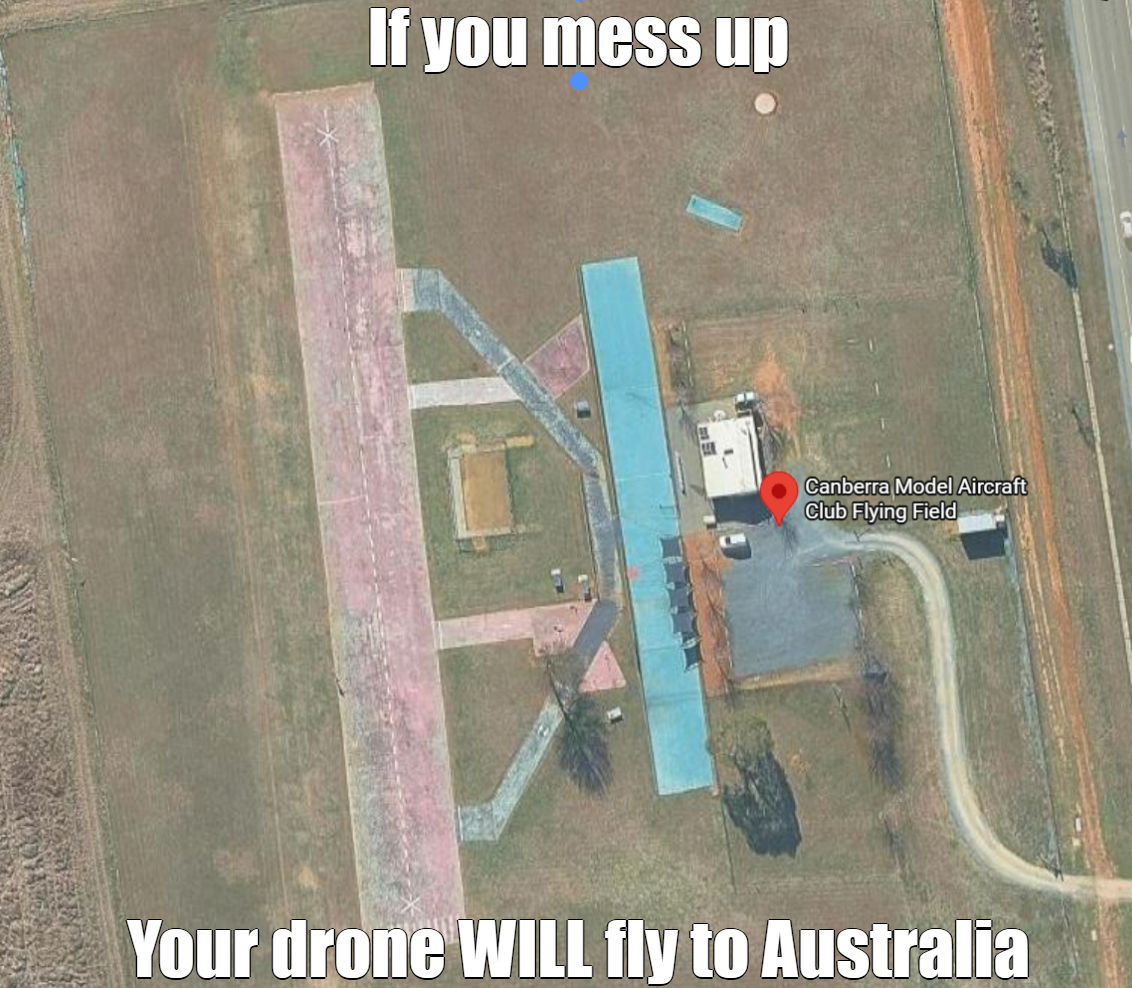
\includegraphics[width=0.7\linewidth]{meme0.png}
        \caption{Figure depicting default GPS origins from the Mavproxy Vicon Module.}
        \label{fig:placeholder3}
    \end{figure}
\vfill
\clearpage


\section{Setting The Foundations}
Now, unlike the previous guide, rather everything is "Plug N Play", in this section things are getting more tricky. Please be patient and follow each step concretely so you setup the system nicely. This allows you to not debug your setup again and again, or thinking you missed a setup step when you're operating your system. Having a good foundation gives you much more comfort when operating your drone, especially if they're fragile to failure! 
\subsection{Hardware Required}
The hardware requirement for applying VICON is much more rigours than operating VICON. You will need to liaise with your corresponding supervisor/client and prepare the following in your own terms: \\
A Linux Running System with both Wifi and Ethernet Capability (Note that when running Linuxm, some laptop's wifi card does not support Ubuntu 18.04, which you will need to reboot the laptop to a newer versrion.)  \\

A Window System running MissionPlanner (QGroundControl is also ok and in fact better as it can be merged into a single system.) \\

Some resilience\\

Drone piloting skillz (Join the Cranfield Drone Flying Club!) \\

There are also hardware reuqirements that are already at the lab: Just find them:\\
A Router or 2: \\

A Ethernet Cable\\

A USB Stick (8Gb or above) 

\subsection{Dual-booting Procedure}
Many of us uses Window for their entire life (Myself included), and it is a struggle to switch from Window to Linux without piror knowledge. Here, I will show you a step by step instruction on Dual-booting your laptop into Linux/Window System. If you already have a Linux System, this section can be skipped. Kindly note that I suggest you ask for a work laptop instead of your personal one as Dual-booting is intrinsicly an "easy to mess up" process. For statistic, 2/12 students in my cohort wiped out all their personal data while dual-booting their personal computer, so warnings to you! 
\clearpage
\subsection{Downloading VICON SDK}
Visit \href{https://www.vicon.com/software/datastream-sdk/}{https://www.vicon.com/software/datastream-sdk/}, the website looks like figure \ref{fig:SDK1}: 
\begin{figure}[H]
    \centering
    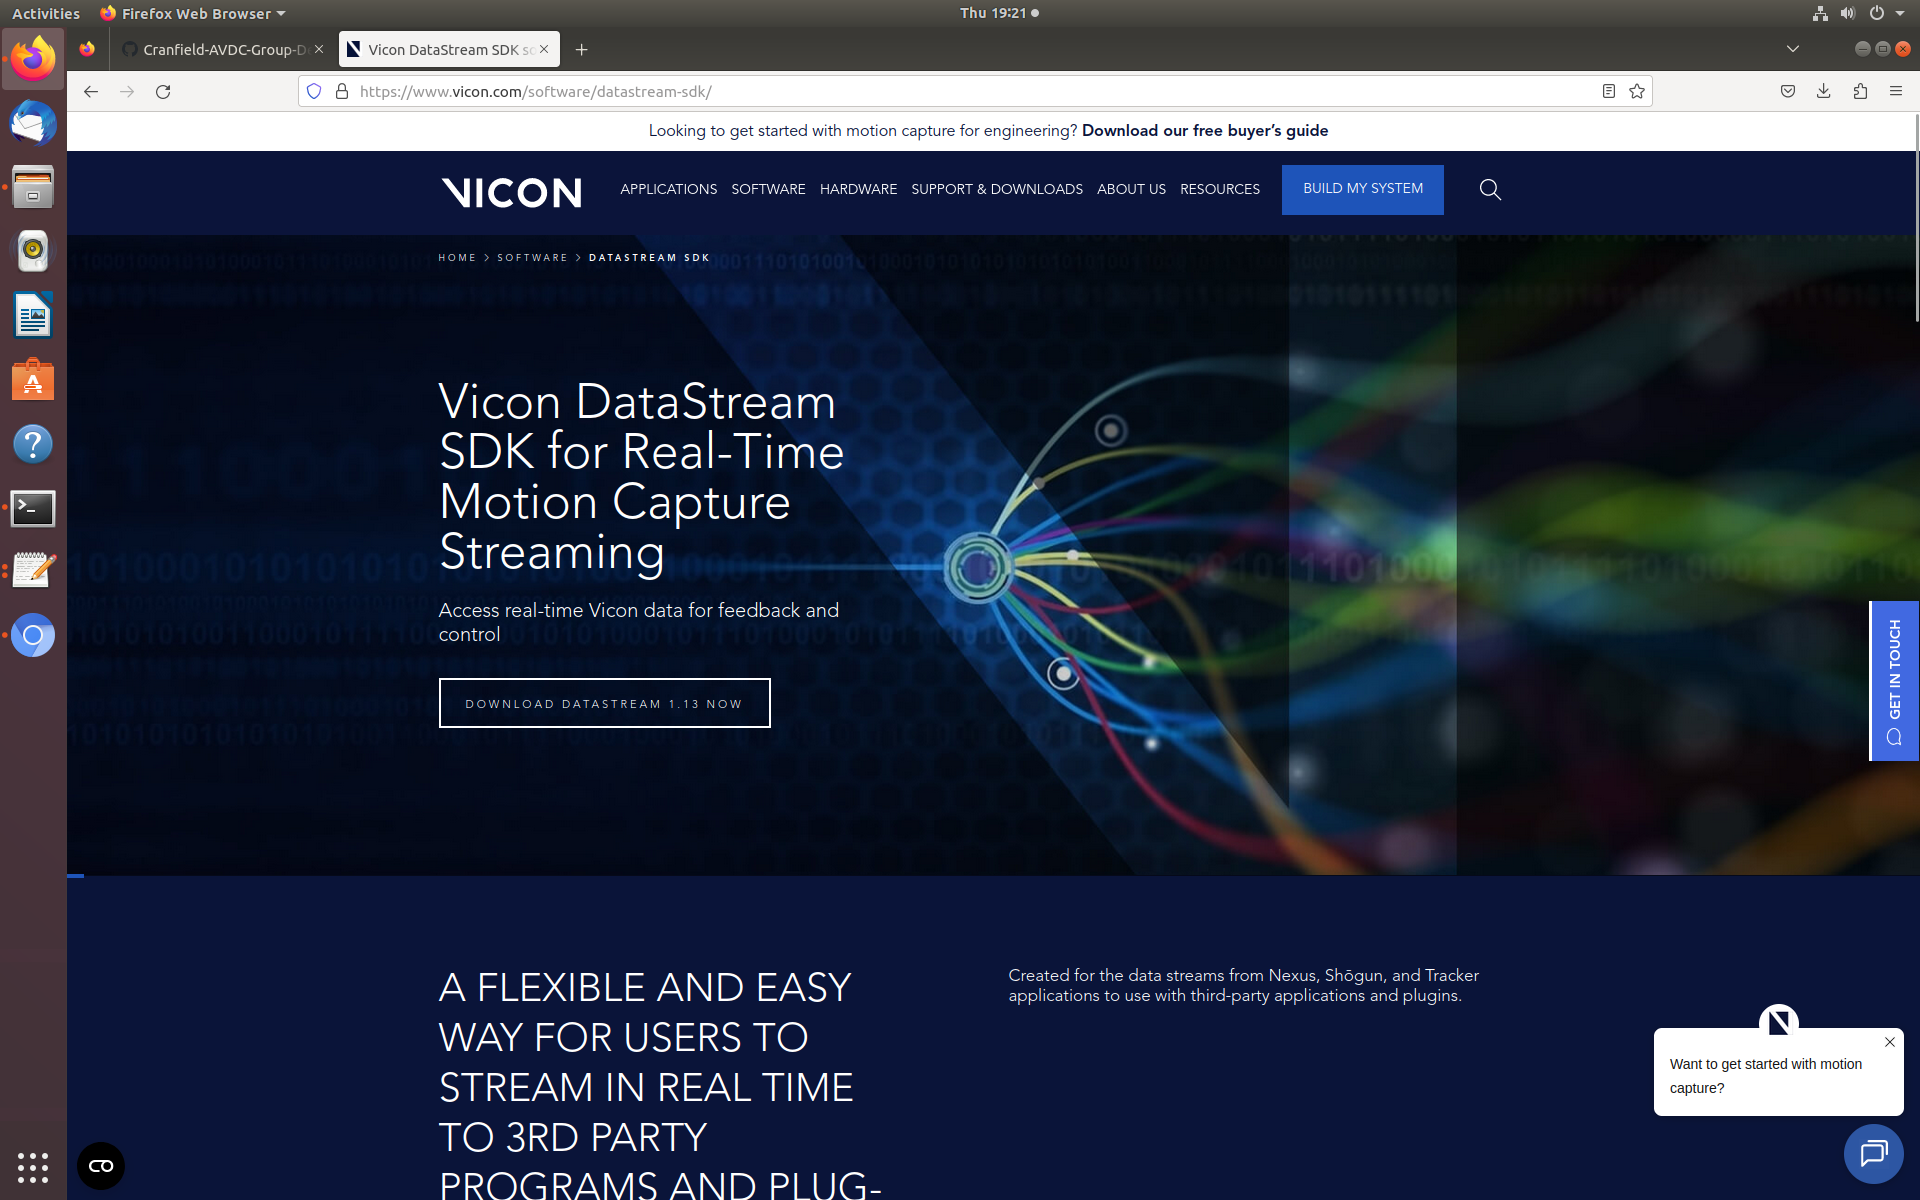
\includegraphics[width=0.9\linewidth]{SDK1.png}
    \caption{VICON SDK Download Website}
    \label{fig:SDK1}
\end{figure}
Scroll down from the page to what is shown in figure \ref{fig:SDK2}:
\begin{figure}[H]
    \centering
    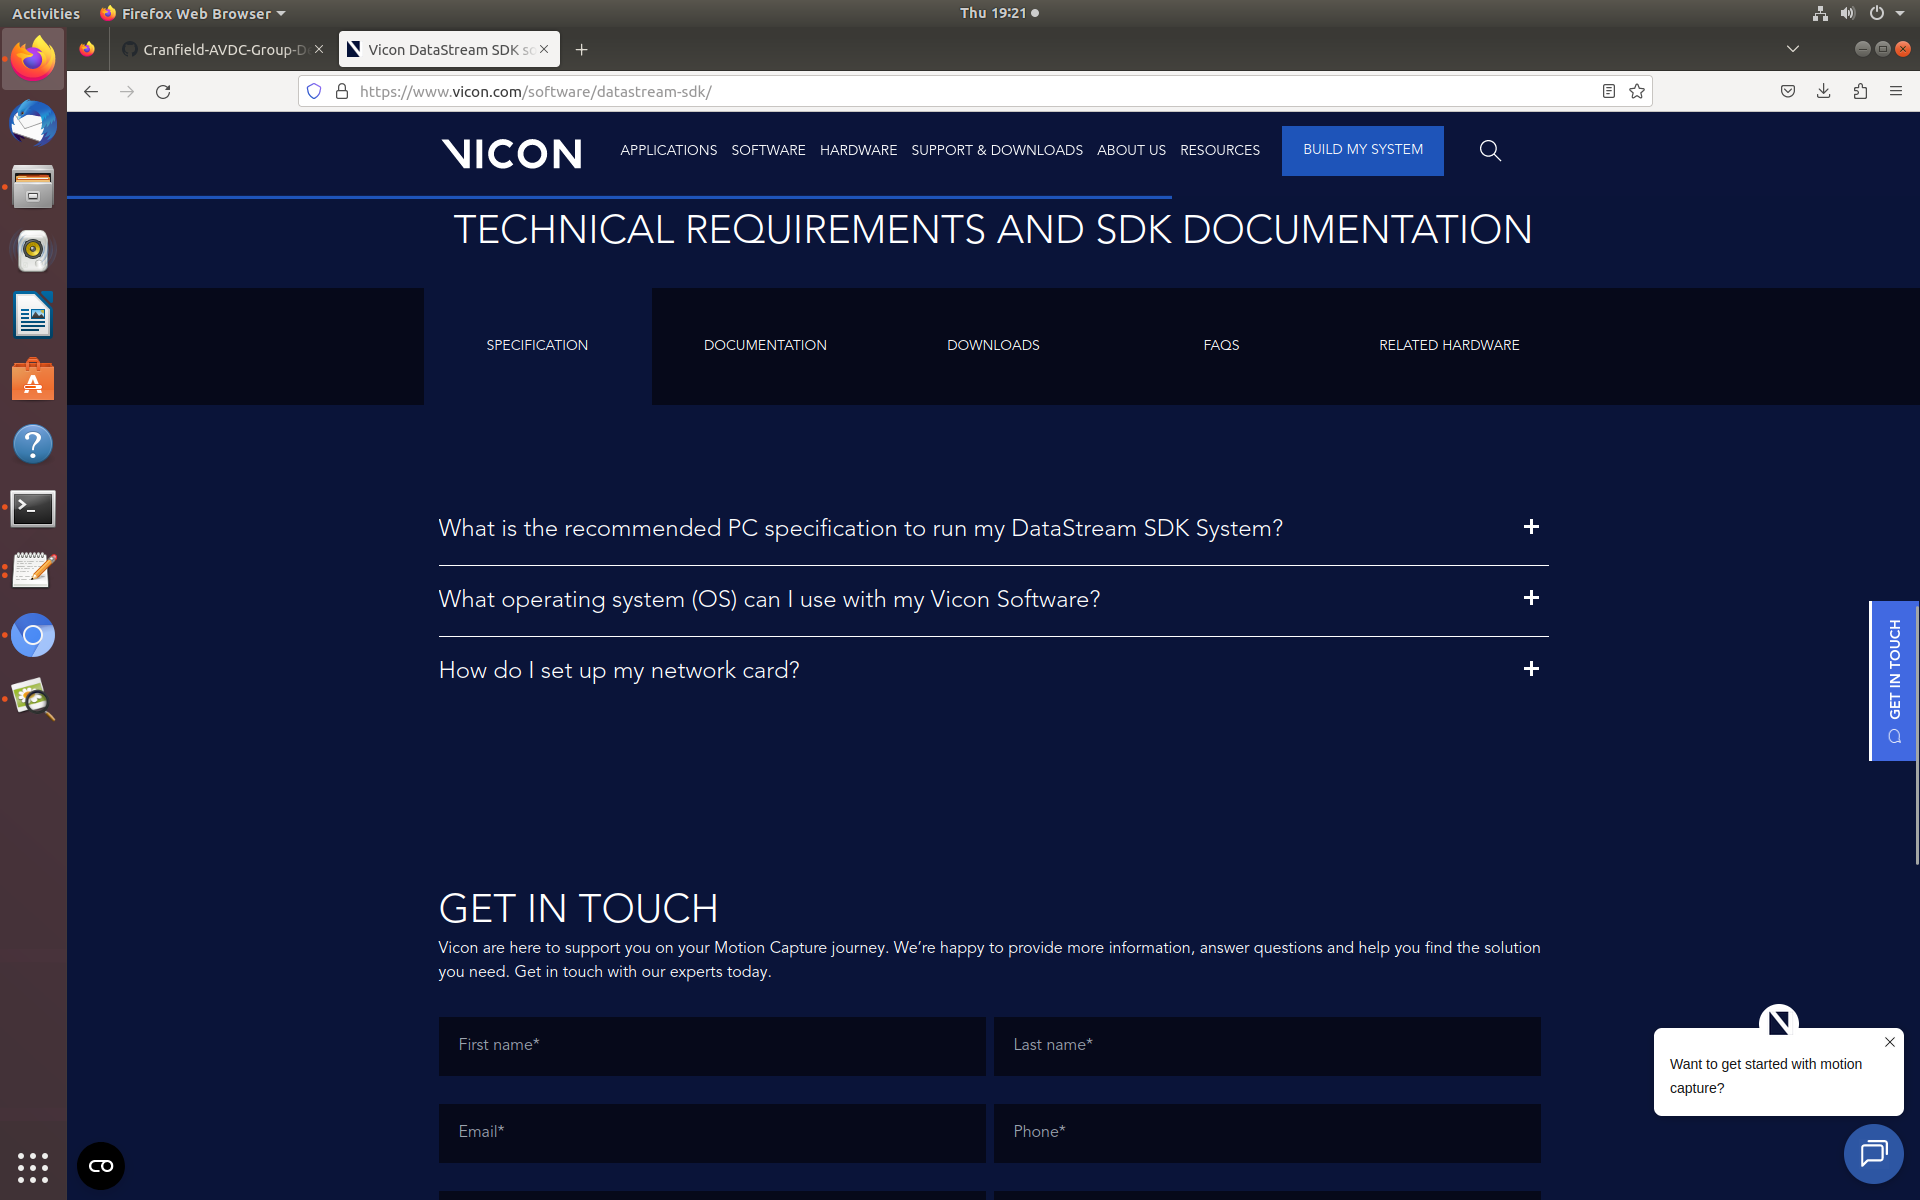
\includegraphics[width=1\linewidth]{SDK2.png}
    \caption{VICON SDK Download Page}
    \label{fig:SDK2}
\end{figure}
Click the downloads tab, install the \textit{Datastream SDK 1.10.0}, write down \textit{an email}, \textit{No} for existing customer, \textit{Tracker} for the Software to Download, click \textit{DOWNLOAD}, as seen in figure \ref{fig:SDK3E}:
\begin{figure}[H]
    \centering
    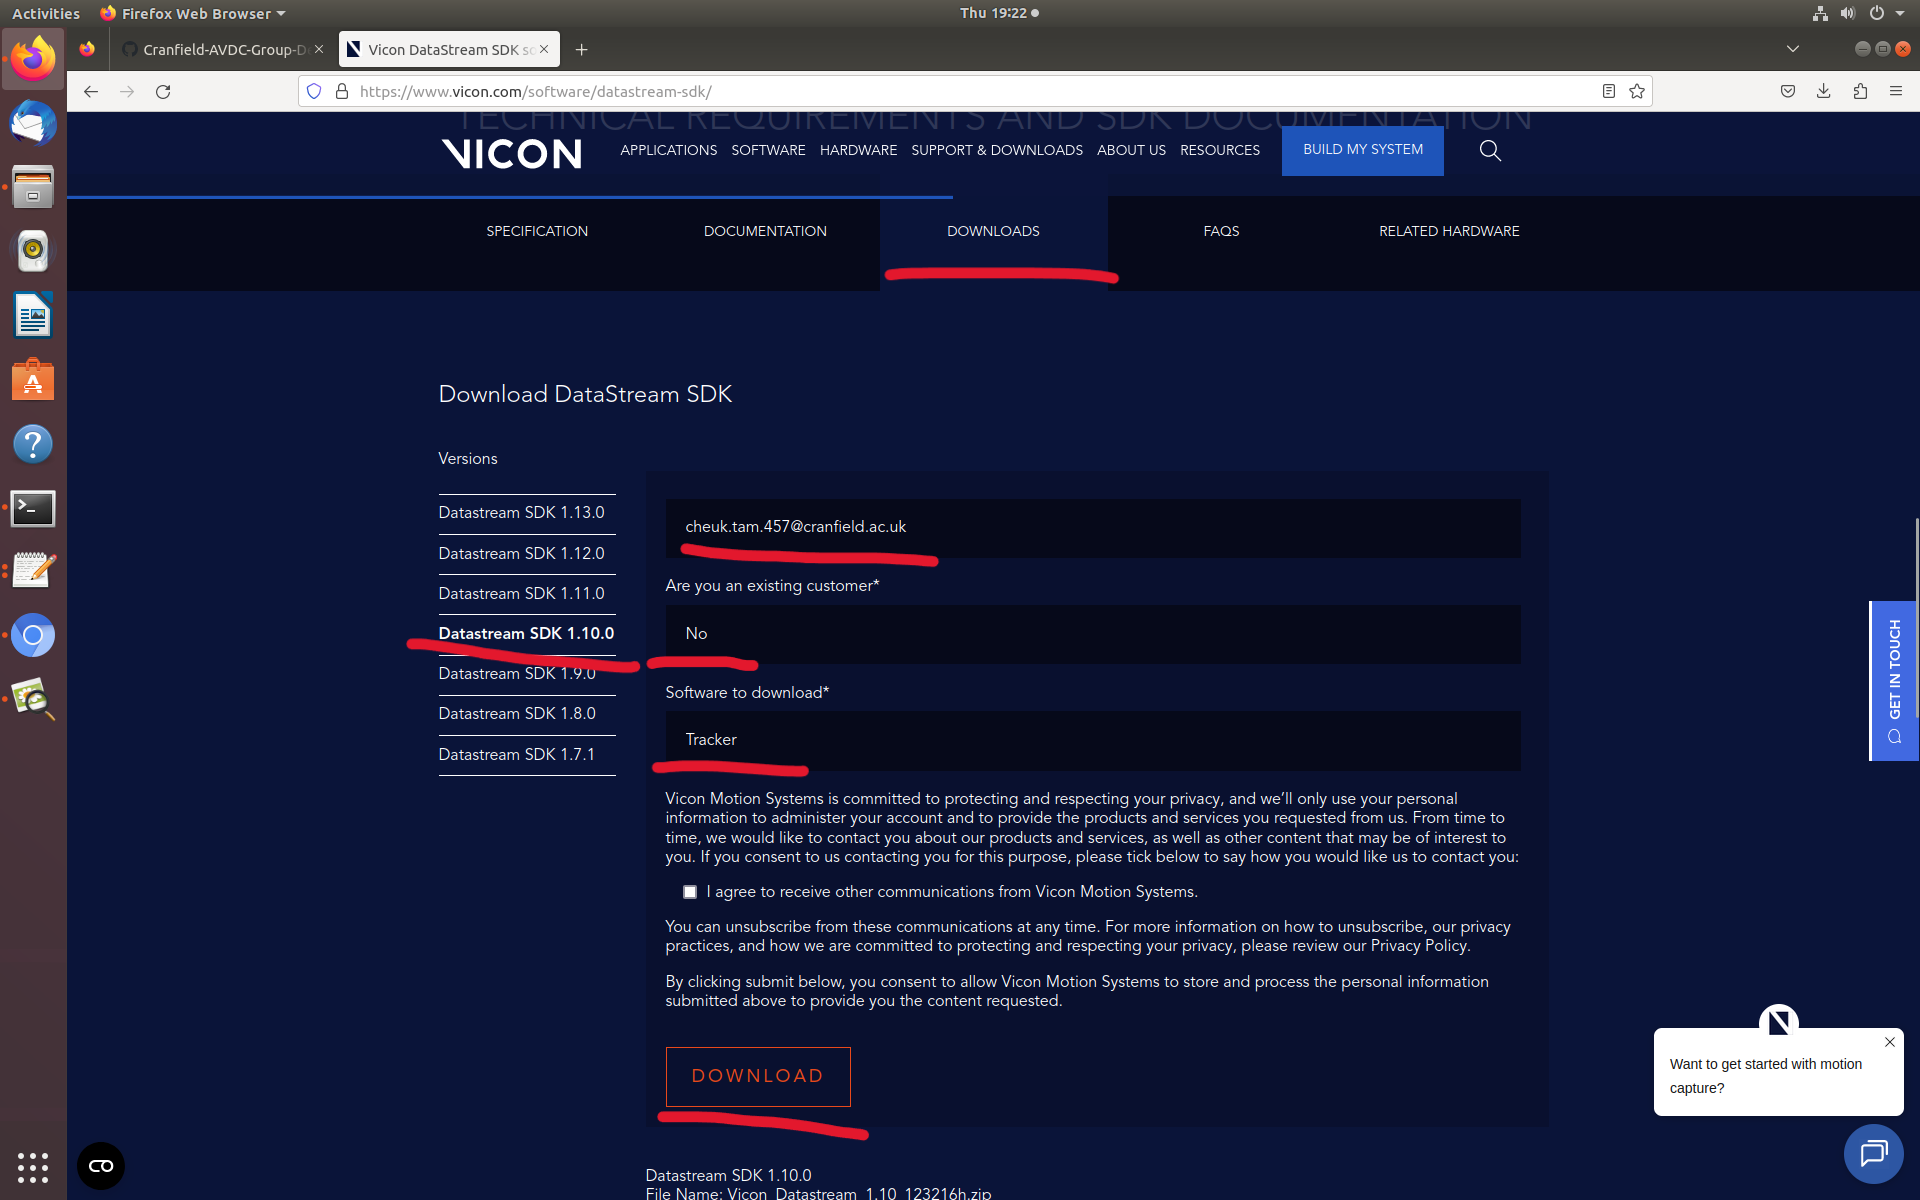
\includegraphics[width=0.9\linewidth]{SDK3E.png}
    \caption{VICON SDK Download Information}
    \label{fig:SDK3E}
\end{figure}
Click \textit{Download} as seen in figure \ref{fig:SDK4}
\begin{figure}[H]
    \centering
    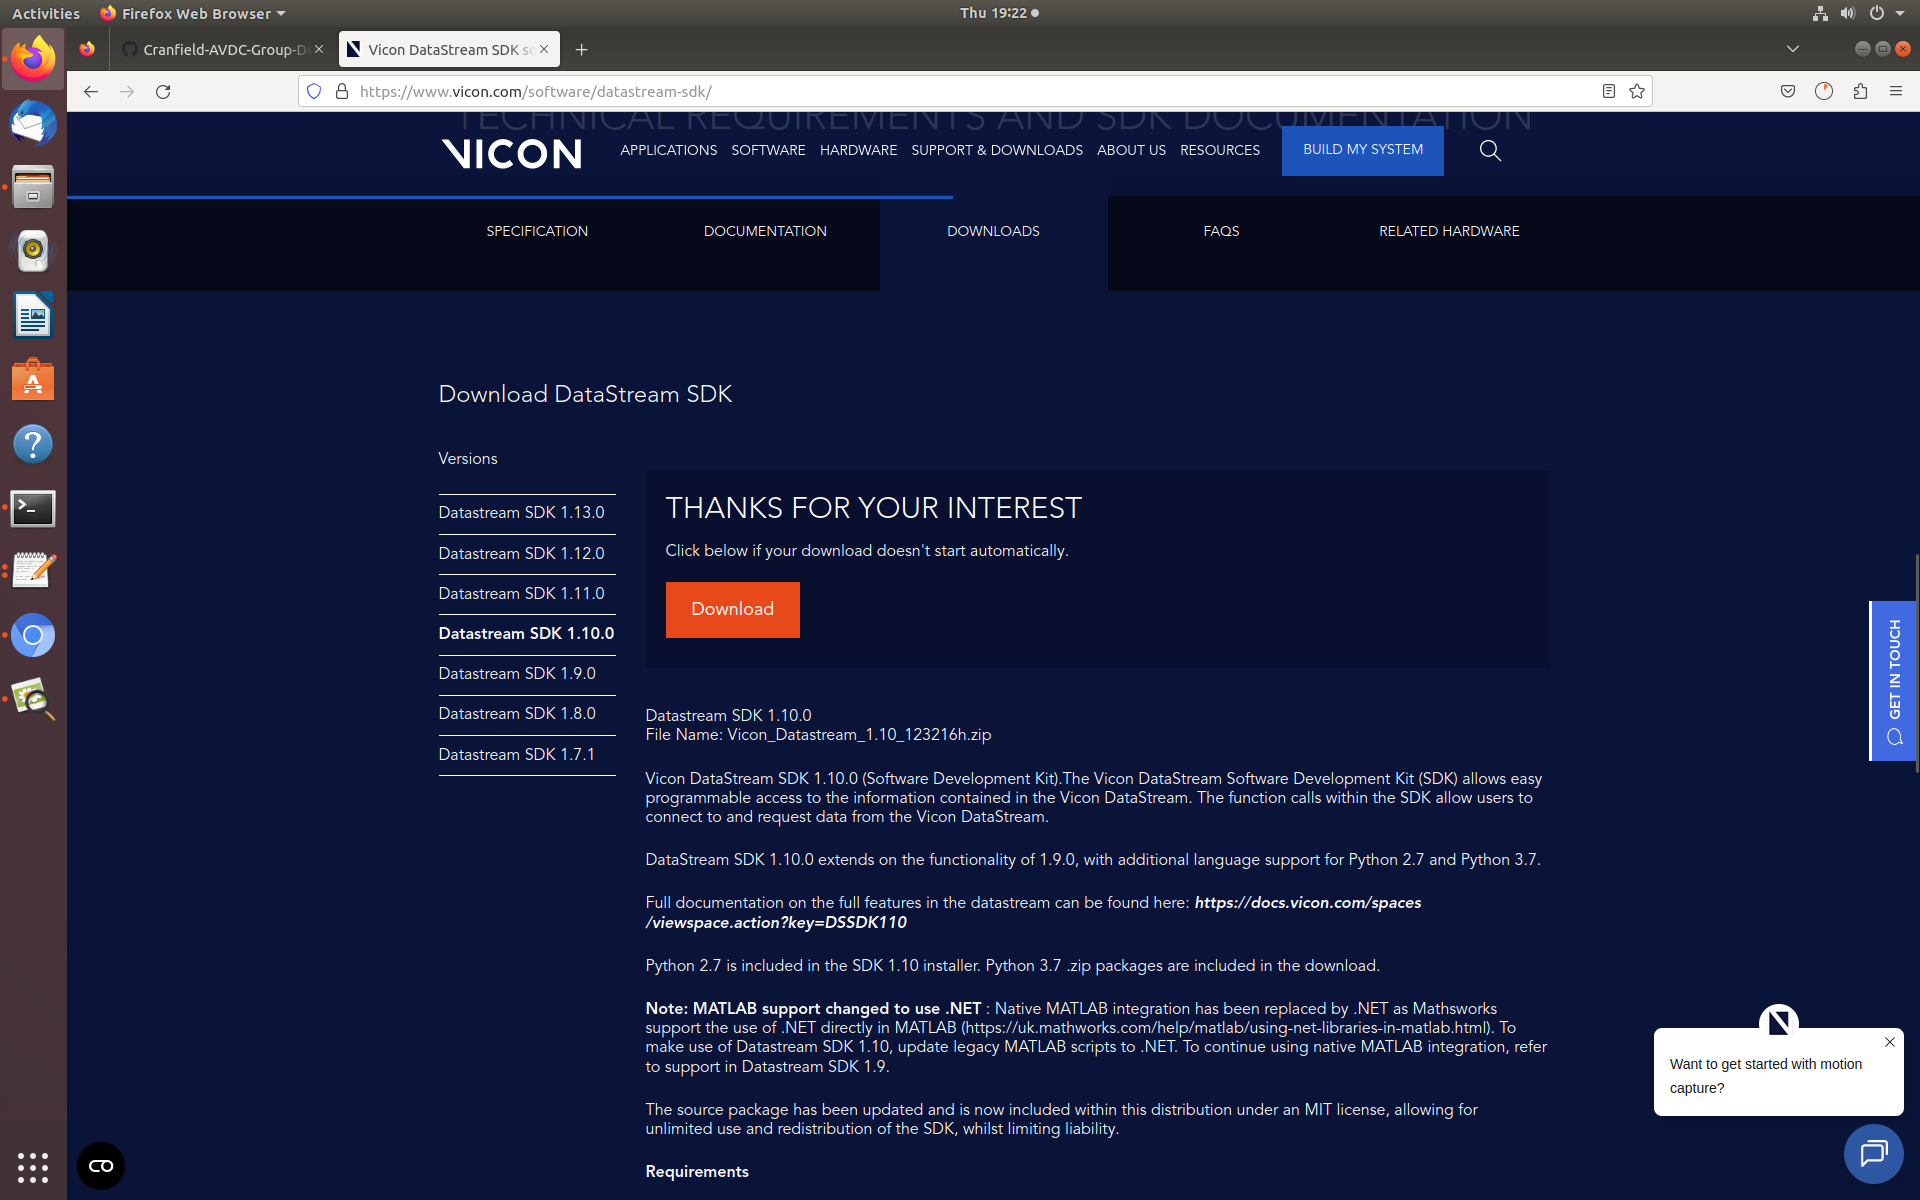
\includegraphics[width=1\linewidth]{SDK4.png}
    \caption{Enter Caption}
    \label{fig:SDK4}
\end{figure}
Navigate to the your \textit{Downloads} Folder, click into \textit{Vicon\_Datastream\_1.10\_123216h.zip}, click into \textit{20200407\_123216h}, into \textit{Linux64}, into \textit{Release}, as seen in figure \ref{fig:SDK59}
\begin{figure}[H]
    \centering
    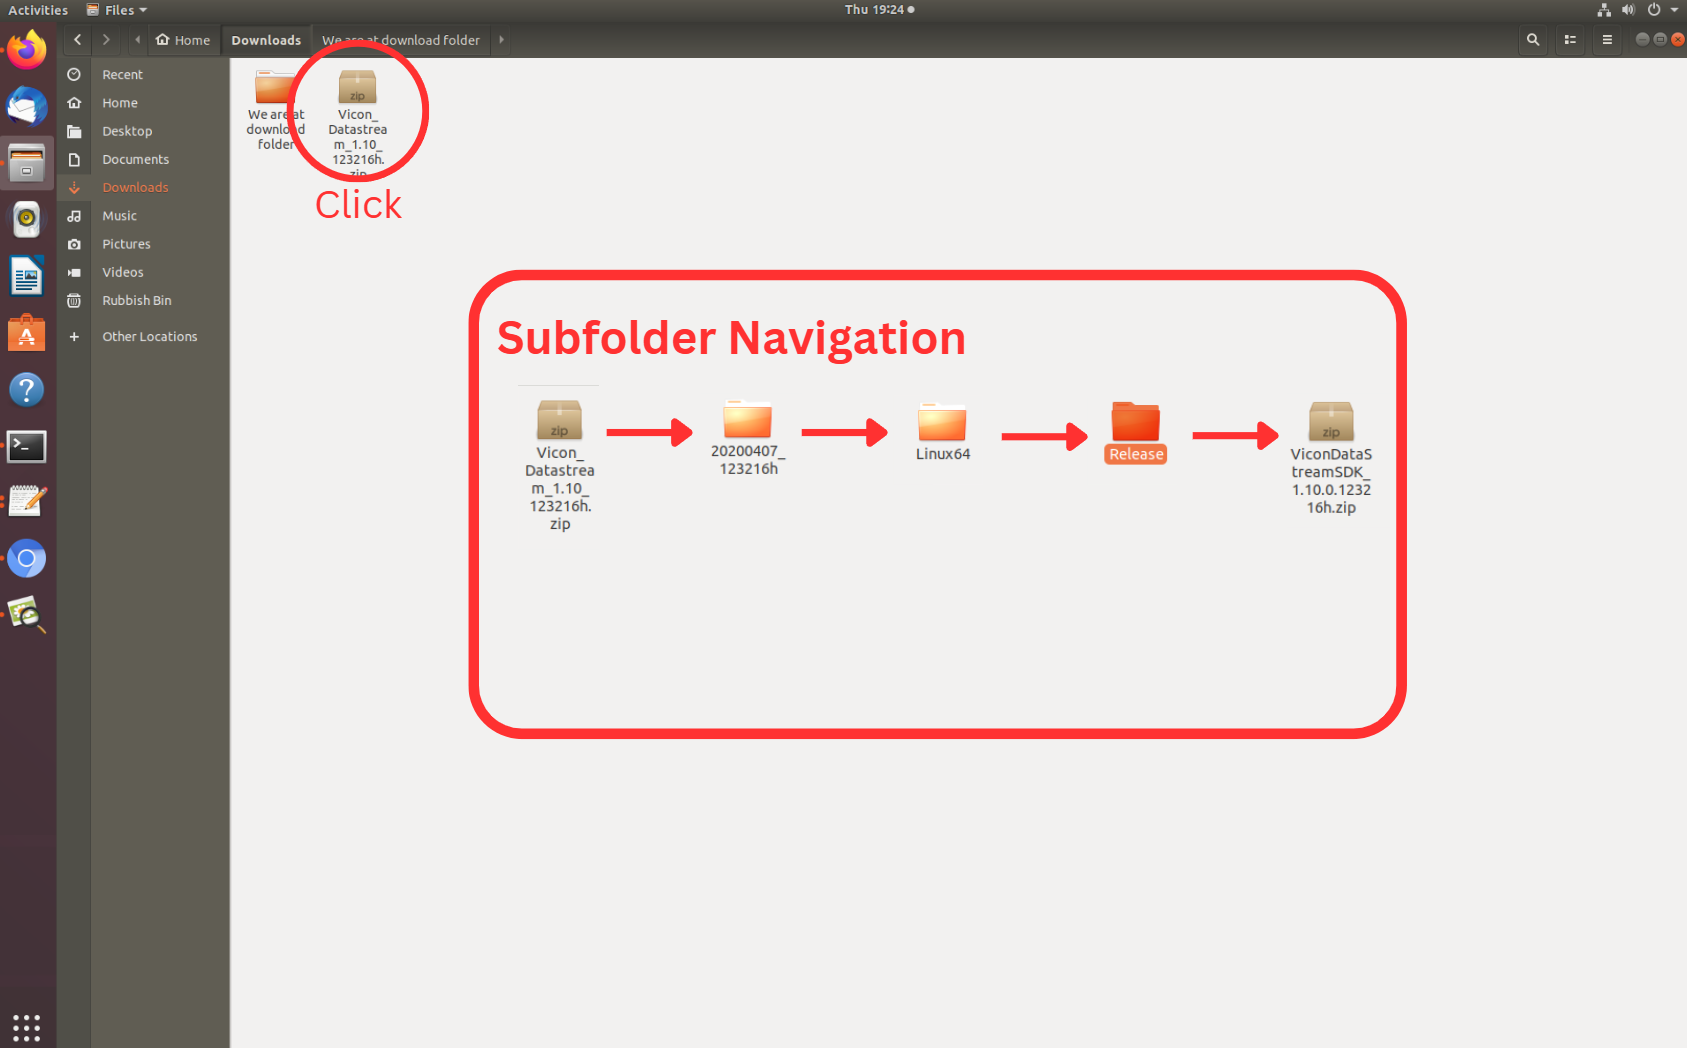
\includegraphics[width=0.9\linewidth]{SDK59.png}
    \caption{Enter Caption}
    \label{fig:SDK59}
\end{figure}
Right click on \textit{ViconDataStreamSDK\_1.10.0.123216h.zip}, extract the file, you should have a file like figure \ref{fig:SDK9}
\begin{figure}[H]
    \centering
    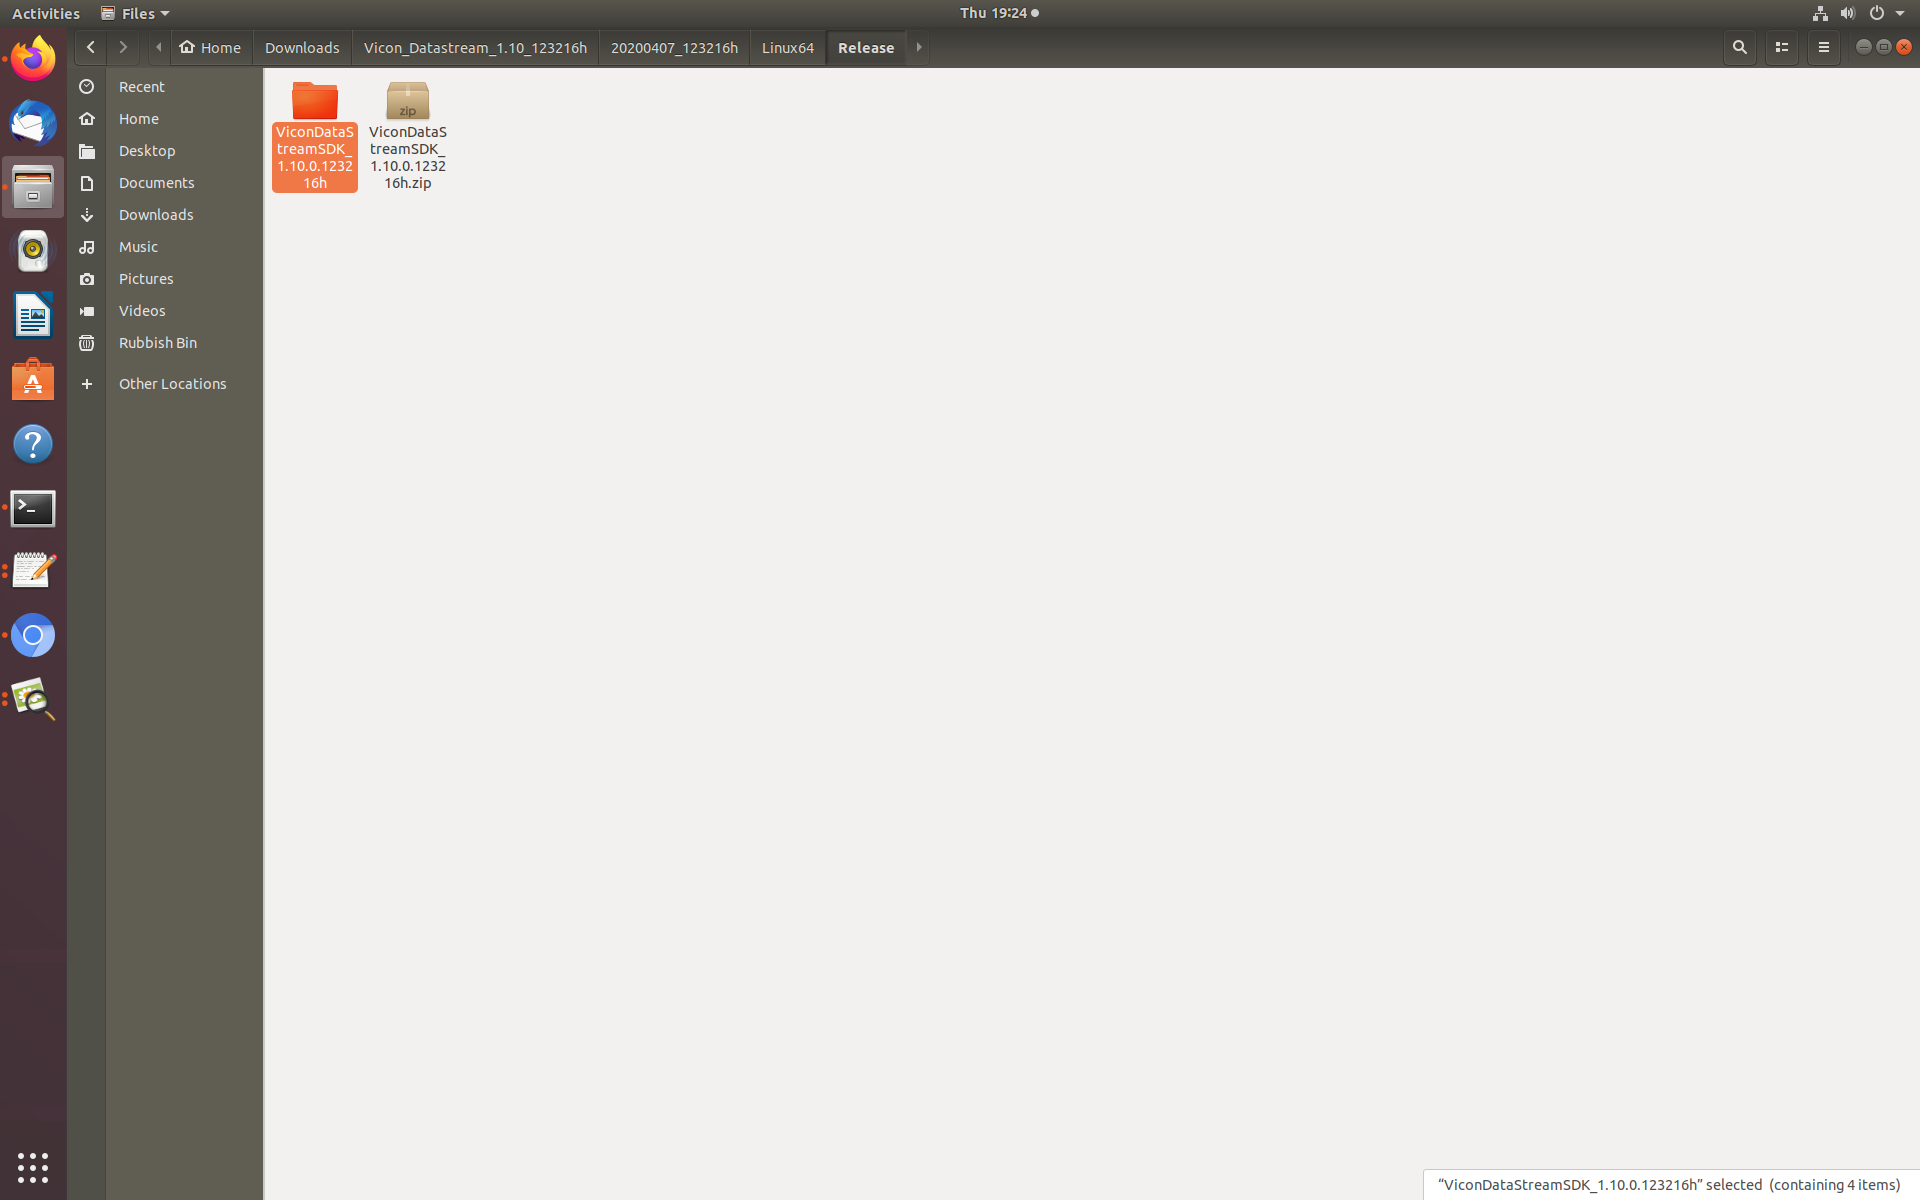
\includegraphics[width=1\linewidth]{SDK9.png}
    \caption{Extracted file of Linux64 Vicon SDK}
    \label{fig:SDK9}
\end{figure}
Drag the extracted file of the Vicon SDK back to the download dictionary as shown in figure \ref{fig:SDK10}
\begin{figure}[H]
    \centering
    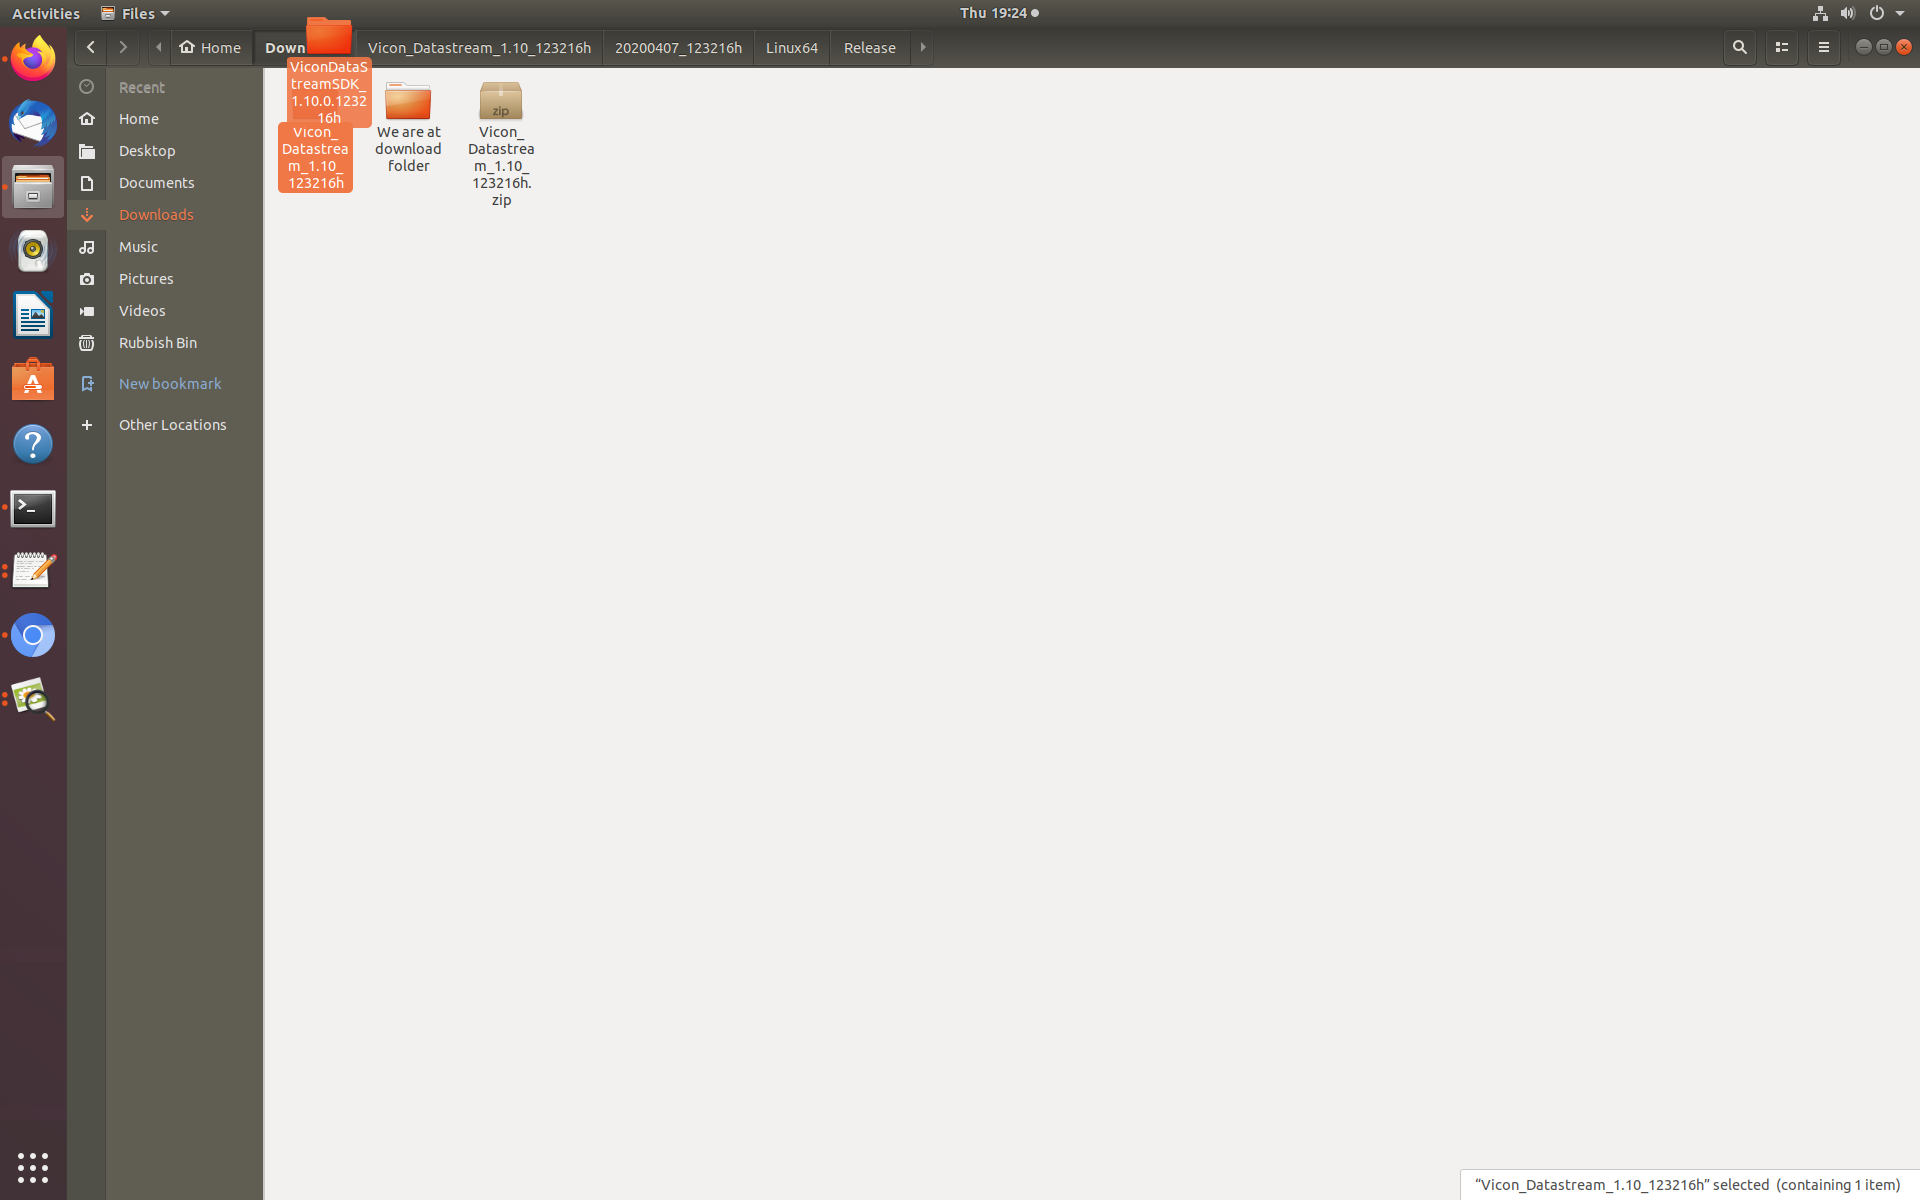
\includegraphics[width=0.9\linewidth]{SDK10.png}
    \caption{Moving Vicon SDK into download folders}
    \label{fig:SDK10}
\end{figure}
Remove the original zip file, they are no longer needed, you should have a singular file as shown in figure \ref{fig:SDK11}.
\begin{figure}[H]
    \centering
    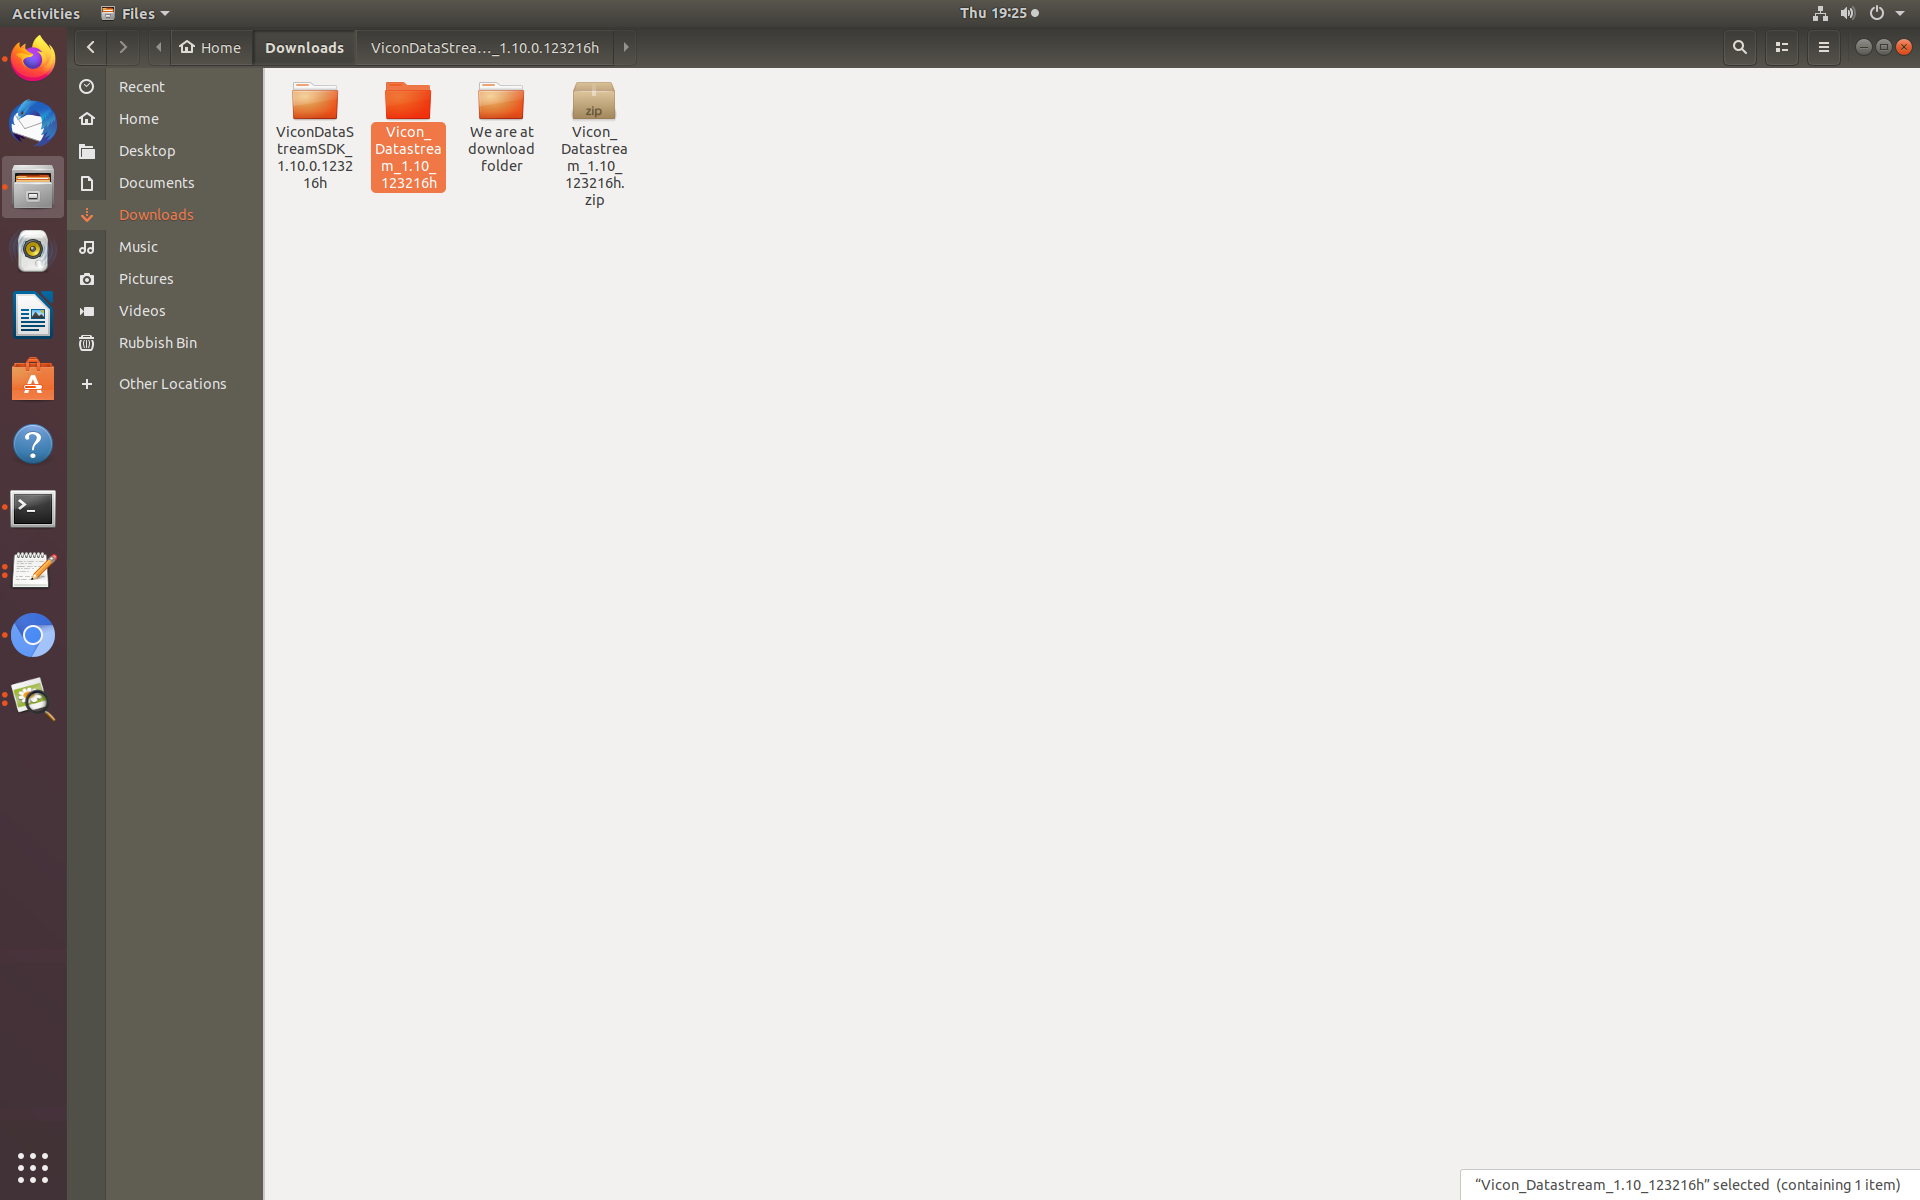
\includegraphics[width=1\linewidth]{SDK11.png}
    \caption{Linux64 Vicon SDK extracted in Downloads Folder}
    \label{fig:SDK11}
\end{figure}
Click into the SDK folder (\textit{ViconDataStreamSDK\_1.10.0.123216h}), you should see 2 zipped files inside it like figure \ref{fig:SDK14}.
\begin{figure}[H]
    \centering
    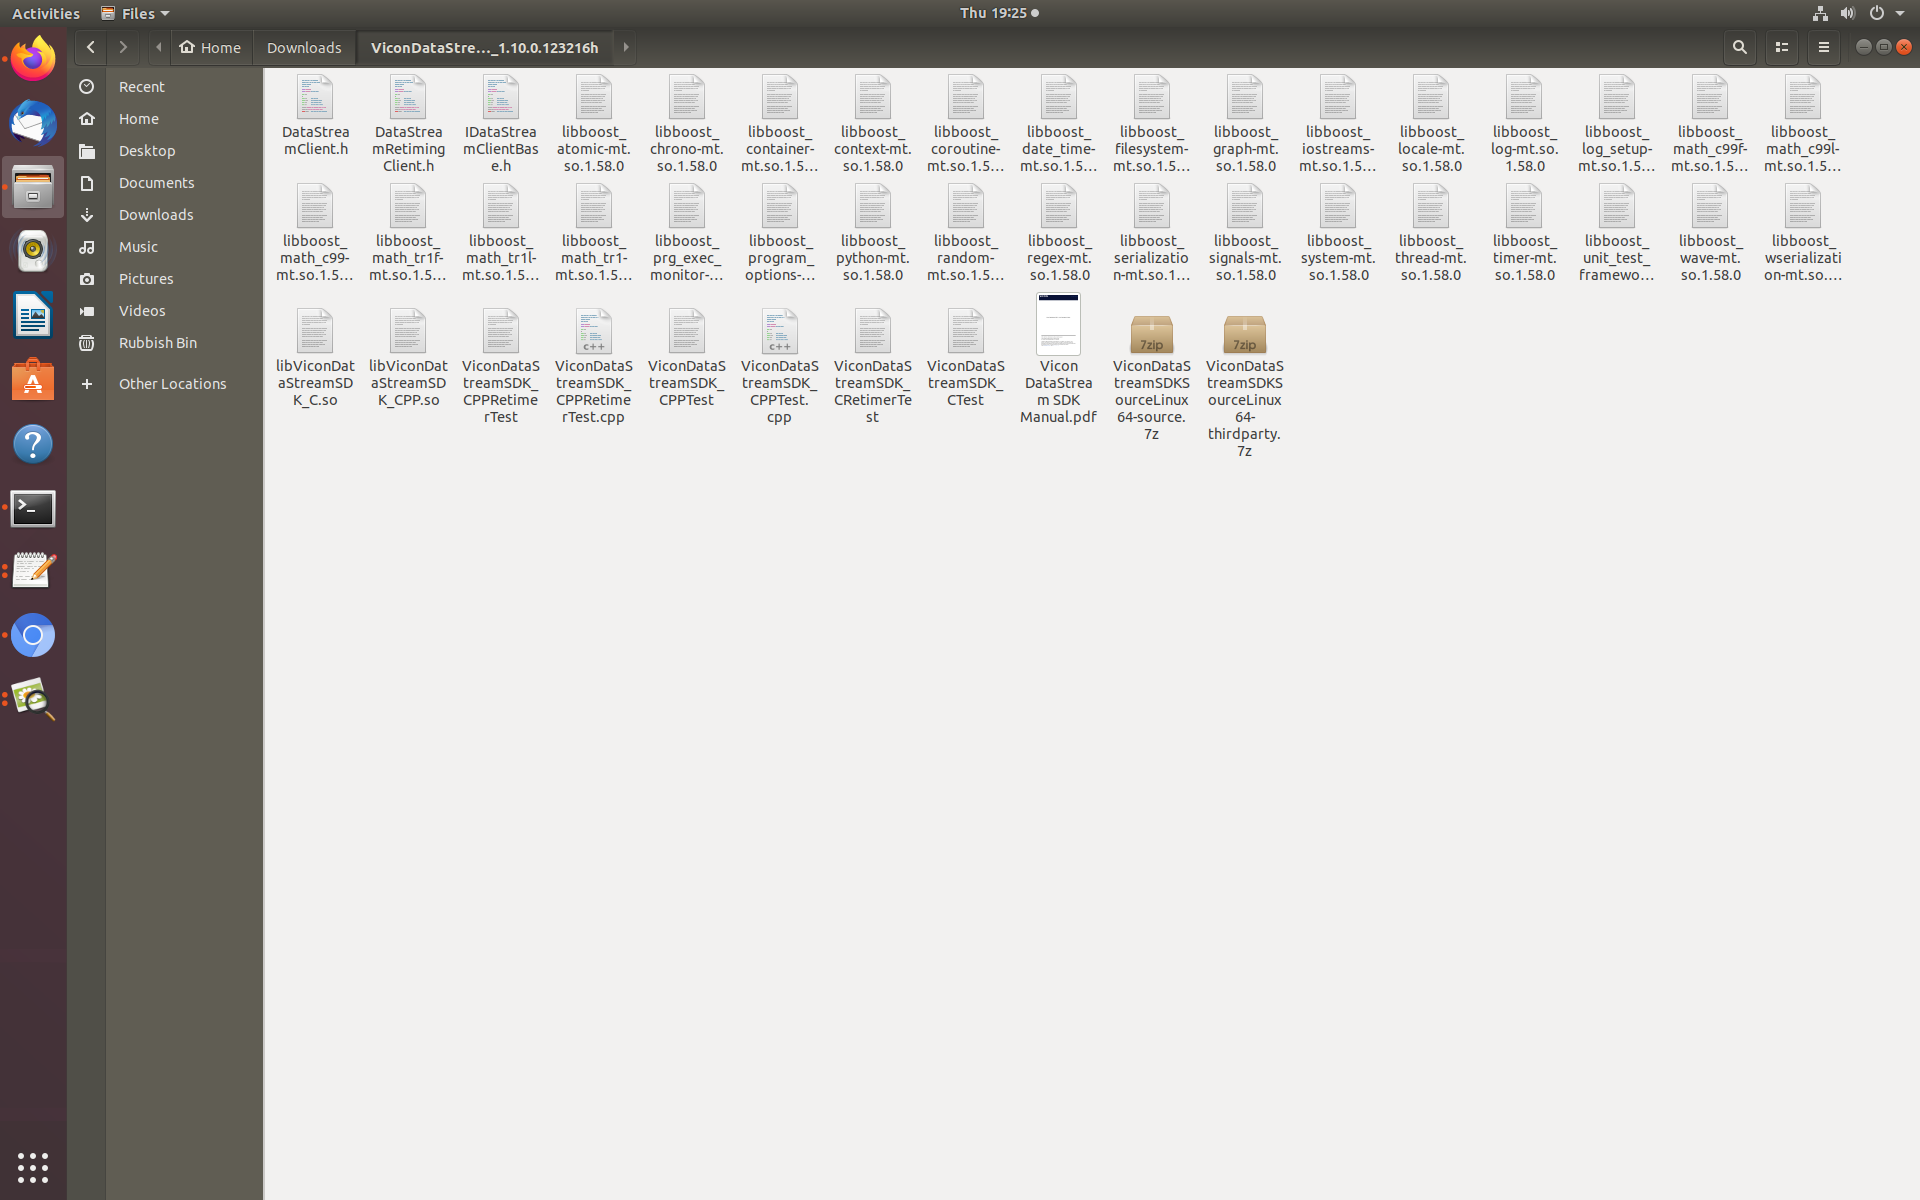
\includegraphics[width=1\linewidth]{SDK14.png}
    \caption{Vicon SDK Folder}
    \label{fig:SDK14}
\end{figure}
Extract the 2 zipped files as shown in figure \ref{fig:SDK15}.
\begin{figure}[H]
    \centering
    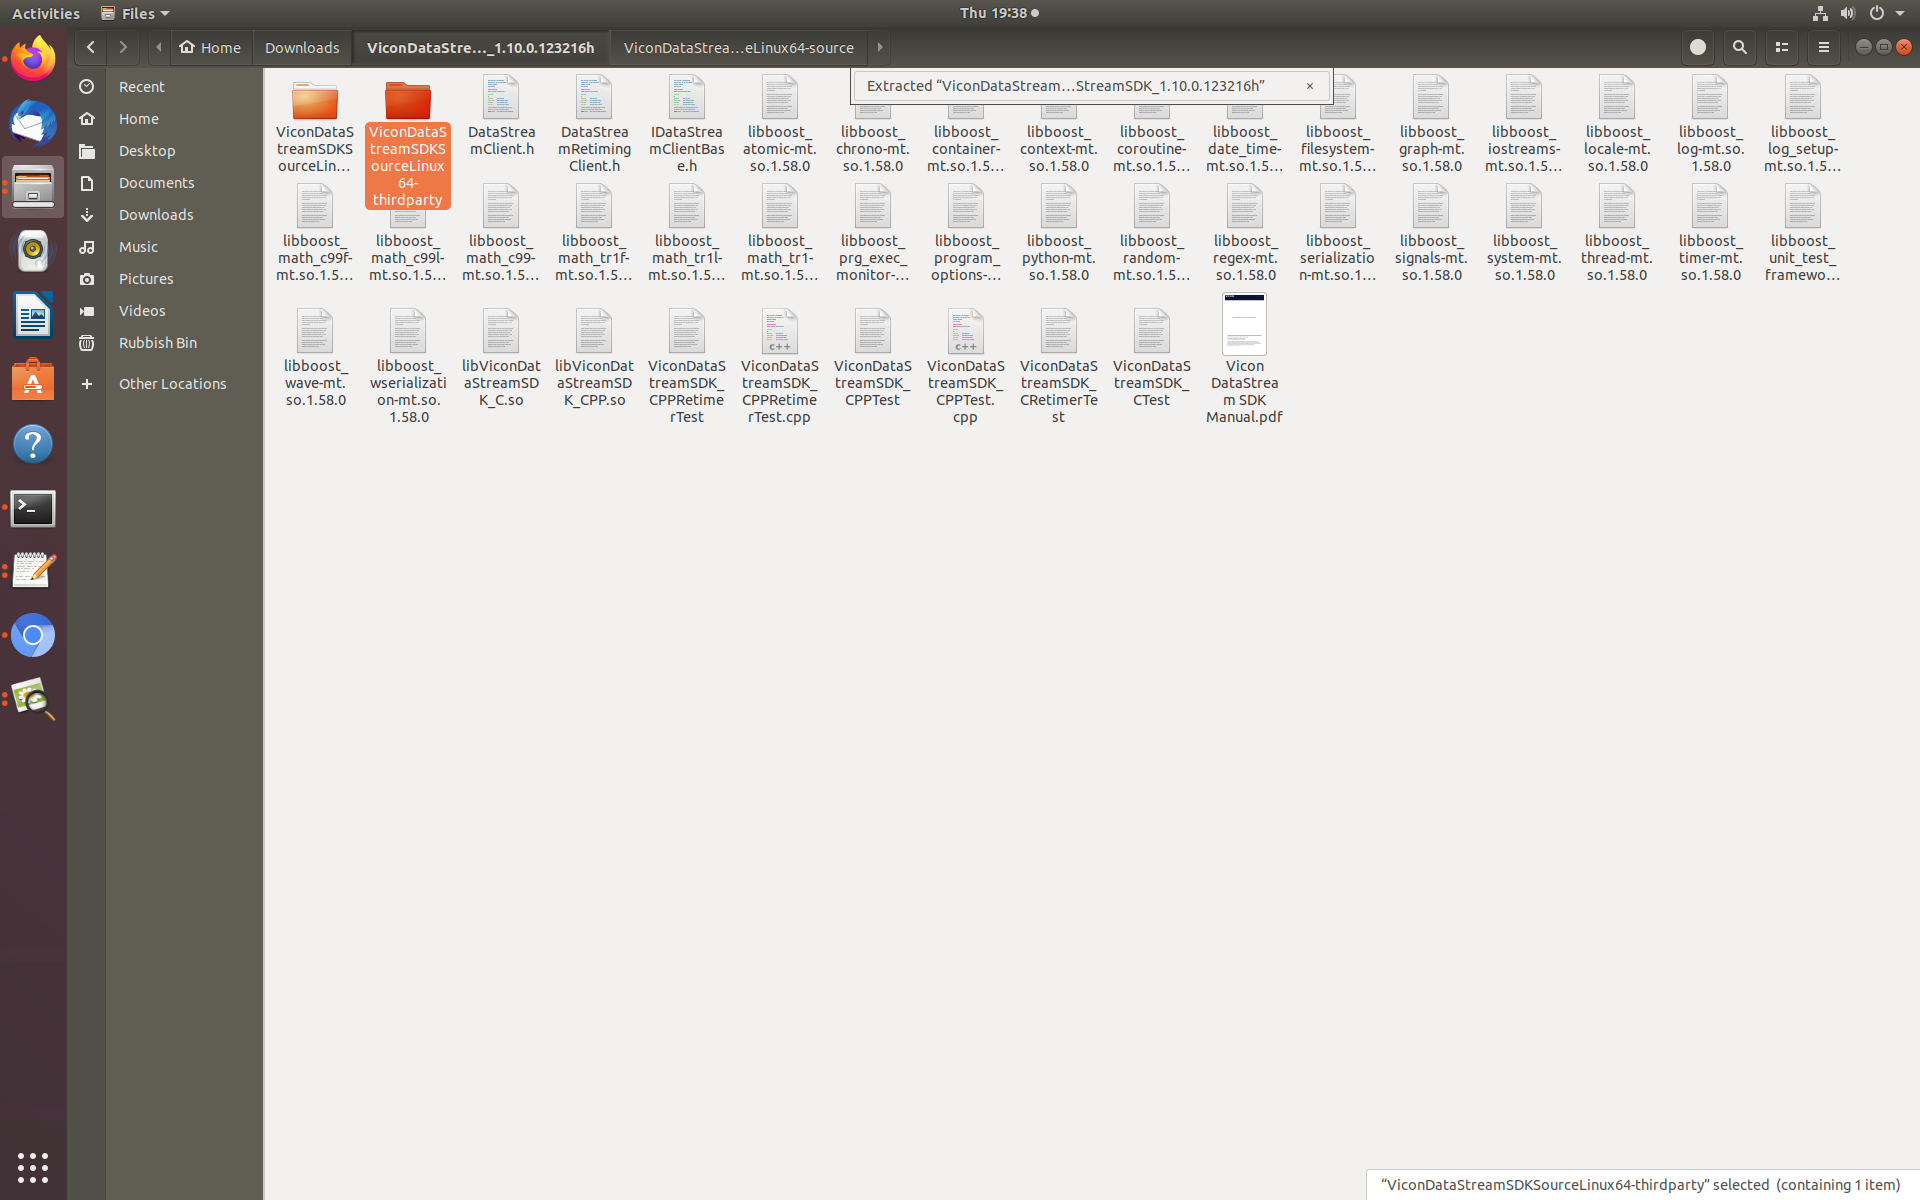
\includegraphics[width=1\linewidth]{SDK15.png}
    \caption{Extracted 2 Subfolders of Vicon SDK Folder}
    \label{fig:SDK15}
\end{figure}

\subsection{Downloading pyvicon}
After SDK is installed, you will need install a custom python script by MathGaron \cite{pyvicon} that bridges the VICON SDK to MAVPROXY. This is installed via
 \href{https://github.com/MathGaron/pyvicon}{https://github.com/MathGaron/pyvicon}, as seen in figure \ref{fig:SDK155}:
 \begin{figure}[H]
     \centering
     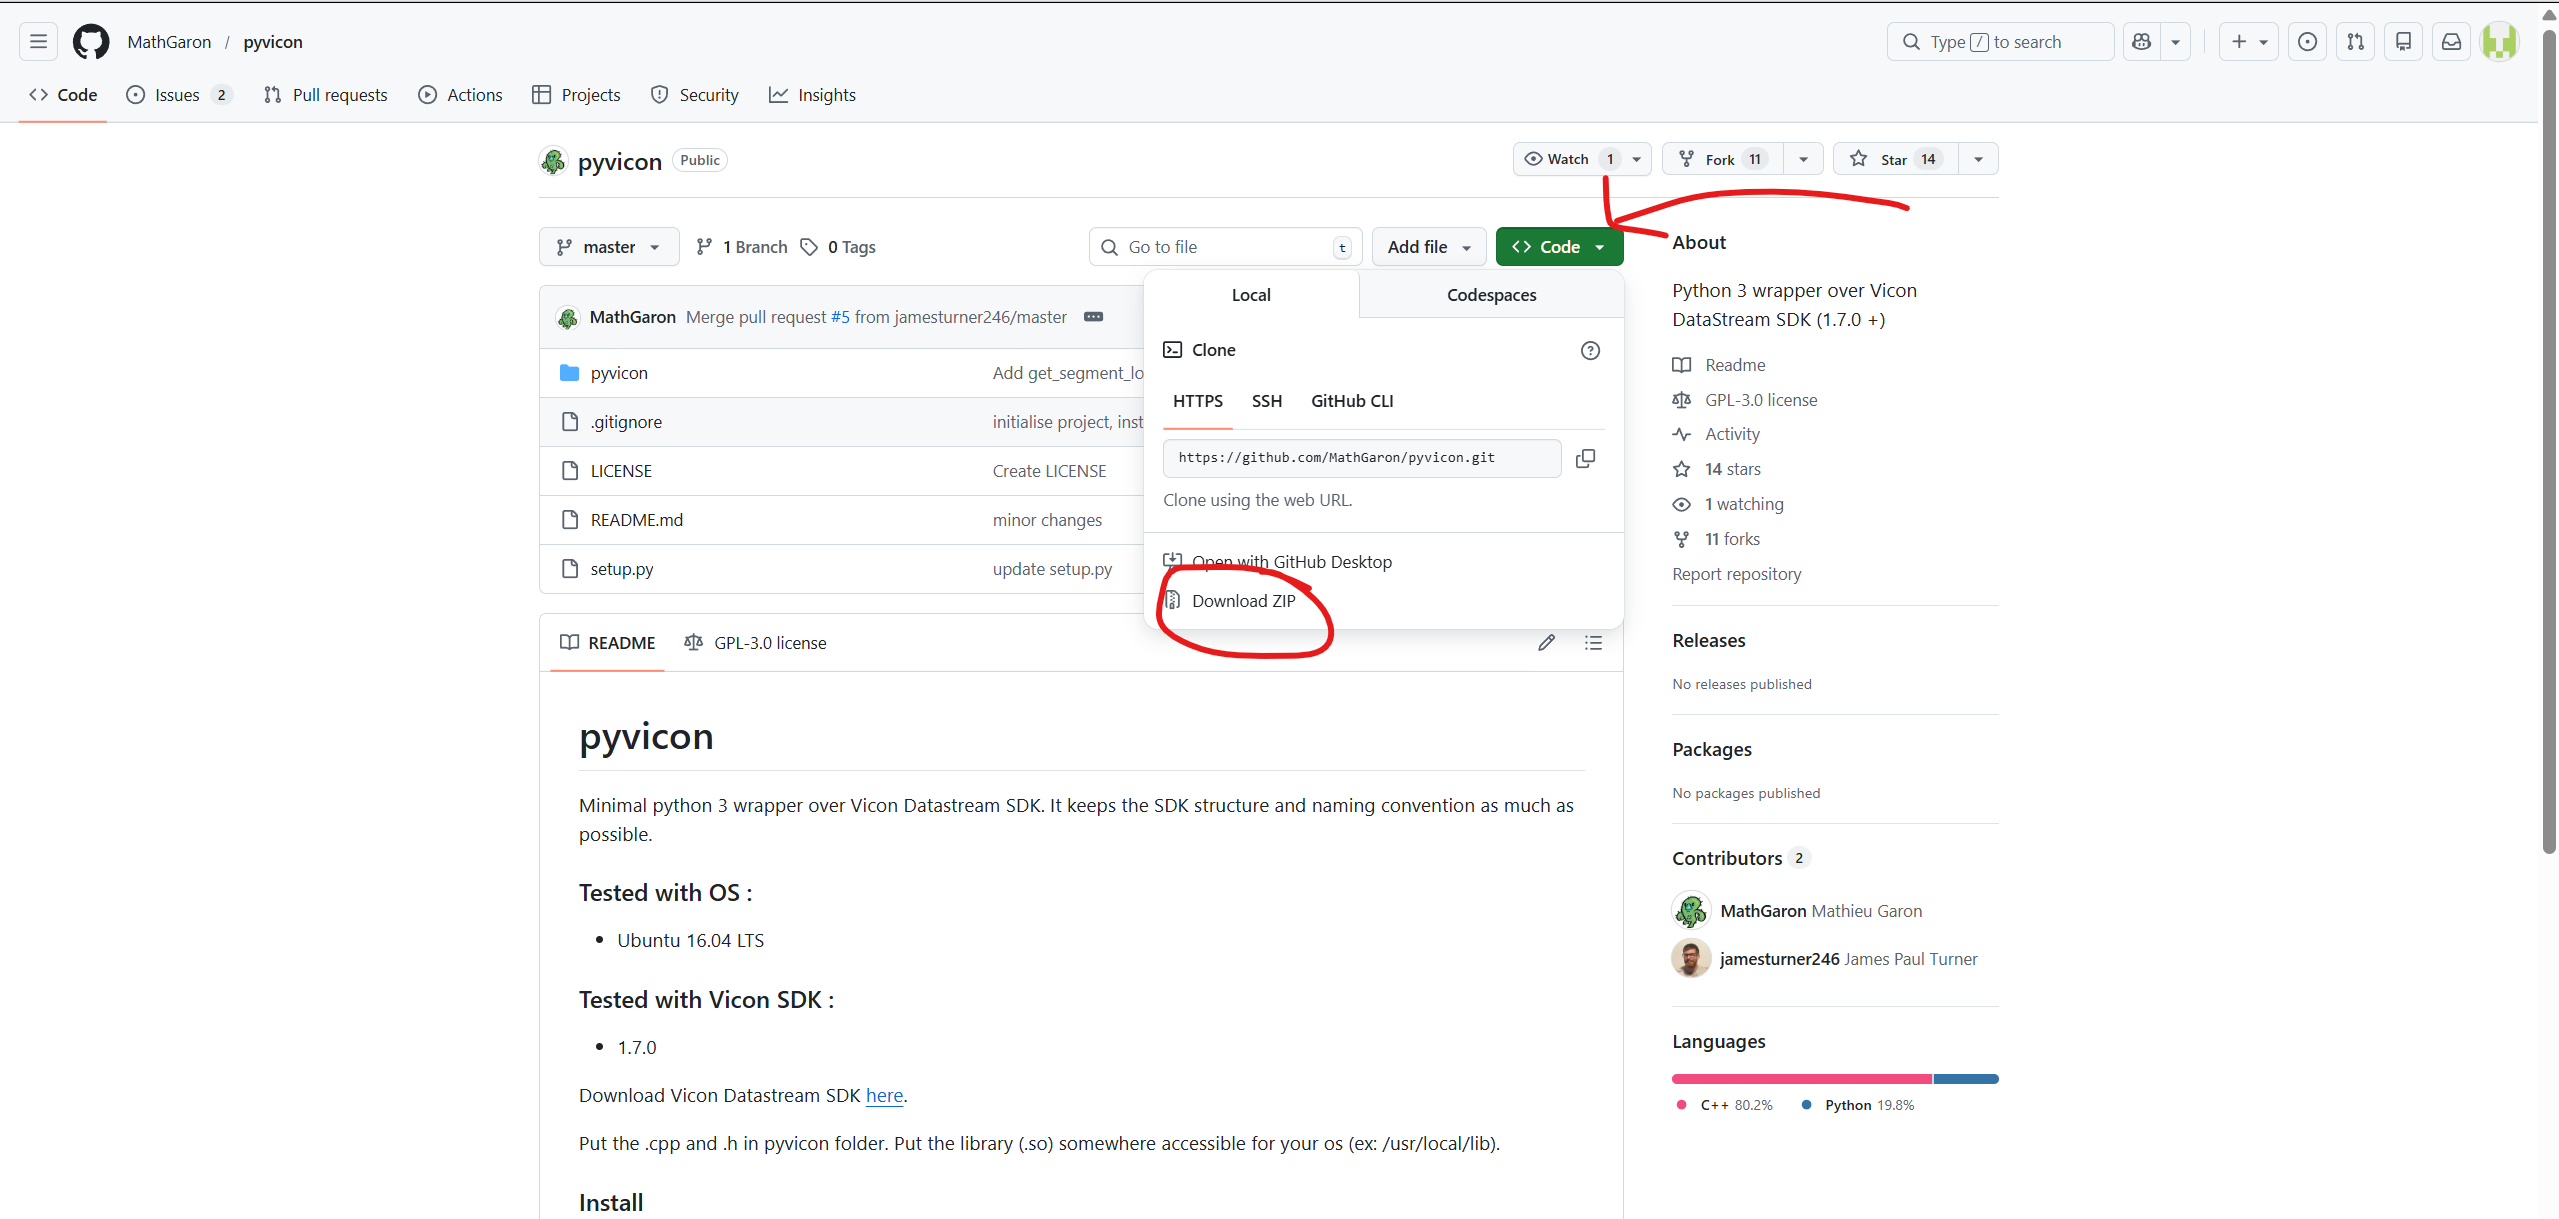
\includegraphics[width=1\linewidth]{SDK155.png}
     \caption{Install the Github file. (Click \textit{Code}, and \textit{Download Zip})}
     \label{fig:SDK155}
\end{figure}
Extract the zipped pyvicon folder into your download folders. Your donwload folder should now have the Vicon SDK folder \& pyvicon folder, as seen in figure \ref{fig:pyvicon1}: 
\begin{figure}[H]
    \centering
    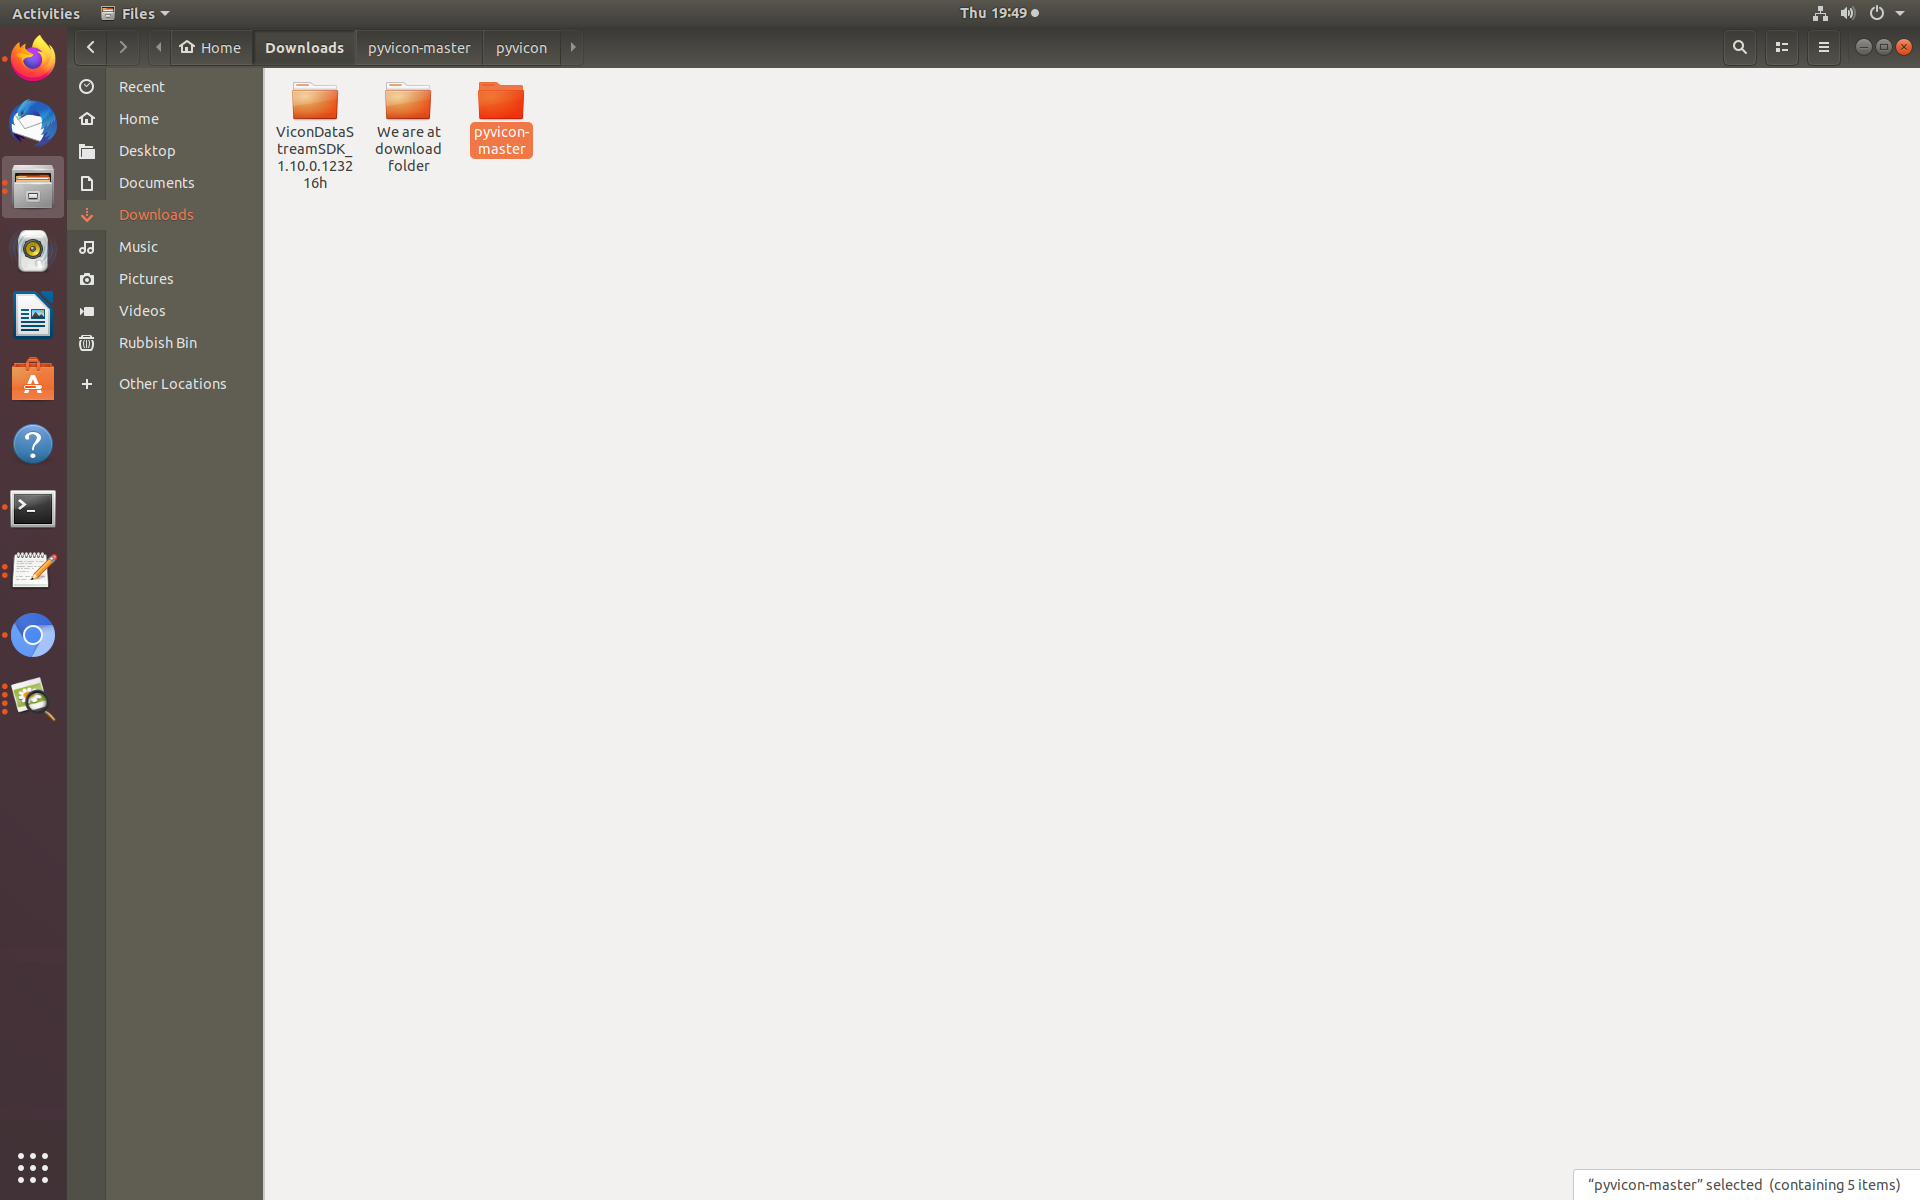
\includegraphics[width=1\linewidth]{pyvicon1.png}
    \caption{Enter Caption}
    \label{fig:pyvicon1}
\end{figure}
\subsection{Merging VICON SDK into pyvicon}
Next, you need to merge the .so files of the VICON SDK into your computer's /user/local/lib. Open your Linux terminal and run a code as shown in \ref{fig:SDK16}.\\
The code is: \\
\begin{lstlisting}[basicstyle=\small\ttfamily, numbers=left,breaklines]{bash}
sudo find ~/Downloads/ViconDataStreamSDK_1.10.0.123216h -name "*.so" -exec cp {} /usr/local/lib/ \;
\end{lstlisting}
You also need to merge the .cpp and h files of Vicon SDK into pyvicon, run this 2 codes in the terminal that automates this, as seen in figure \ref{fig:SDK195}:
\begin{lstlisting}[basicstyle=\small\ttfamily, numbers=left,breaklines]{bash}
sudo find ~/Downloads/ViconDataStreamSDK_1.10.0.123216h -name "*.cpp" -exec mv {} ~/Downloads/pyvicon-master/pyvicon/ \;
\end{lstlisting}

\begin{lstlisting}[basicstyle=\small\ttfamily, numbers=left,breaklines]{bash}
sudo find ~/Downloads/ViconDataStreamSDK_1.10.0.123216h -name "*.cpp" -exec mv {} ~/Downloads/pyvicon-master/pyvicon/ \;
\end{lstlisting}
\begin{figure}[H]
    \centering
    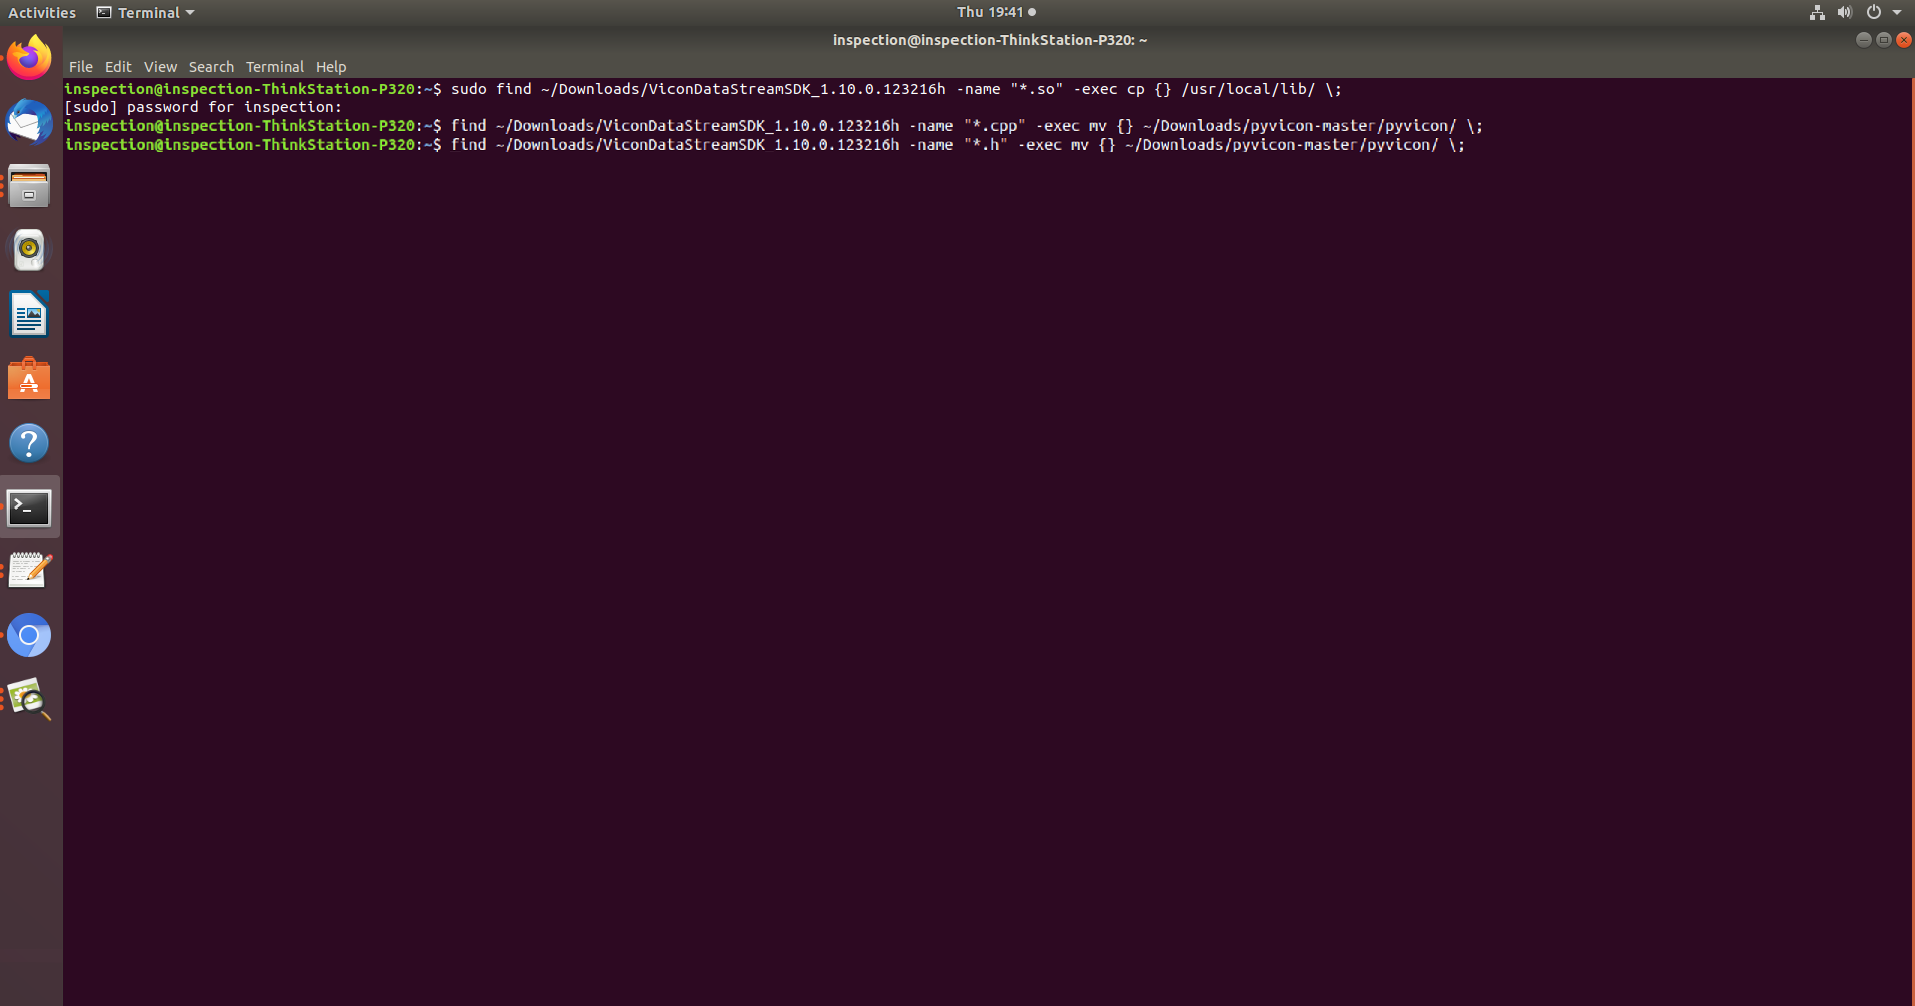
\includegraphics[width=1\linewidth]{SDK195.png}
    \caption{File merging codes}
    \label{fig:SDK195}
\end{figure}
\subsection{Setting up pyvicon}
Once the files are merged, we can run the python script setup for pyvicon. (Please install python3 in Linux if you haven't!) 
Run: 
\begin{lstlisting}[basicstyle=\small\ttfamily, numbers=left,breaklines]{bash}
sudo python3 setup.py install
\end{lstlisting}

You will also need to add \textit{$\sim$/.local/bin} to \textit{PATH} for pyvicon:
\begin{lstlisting}
echo 'export PATH="$HOME/.local/bin:$PATH"' >> ~/.bashrc && source ~/.bashrc
\end{lstlisting}
Both commands can be seen in figure \ref{fig:pyvicon4}
\begin{figure}[H]
    \centering
    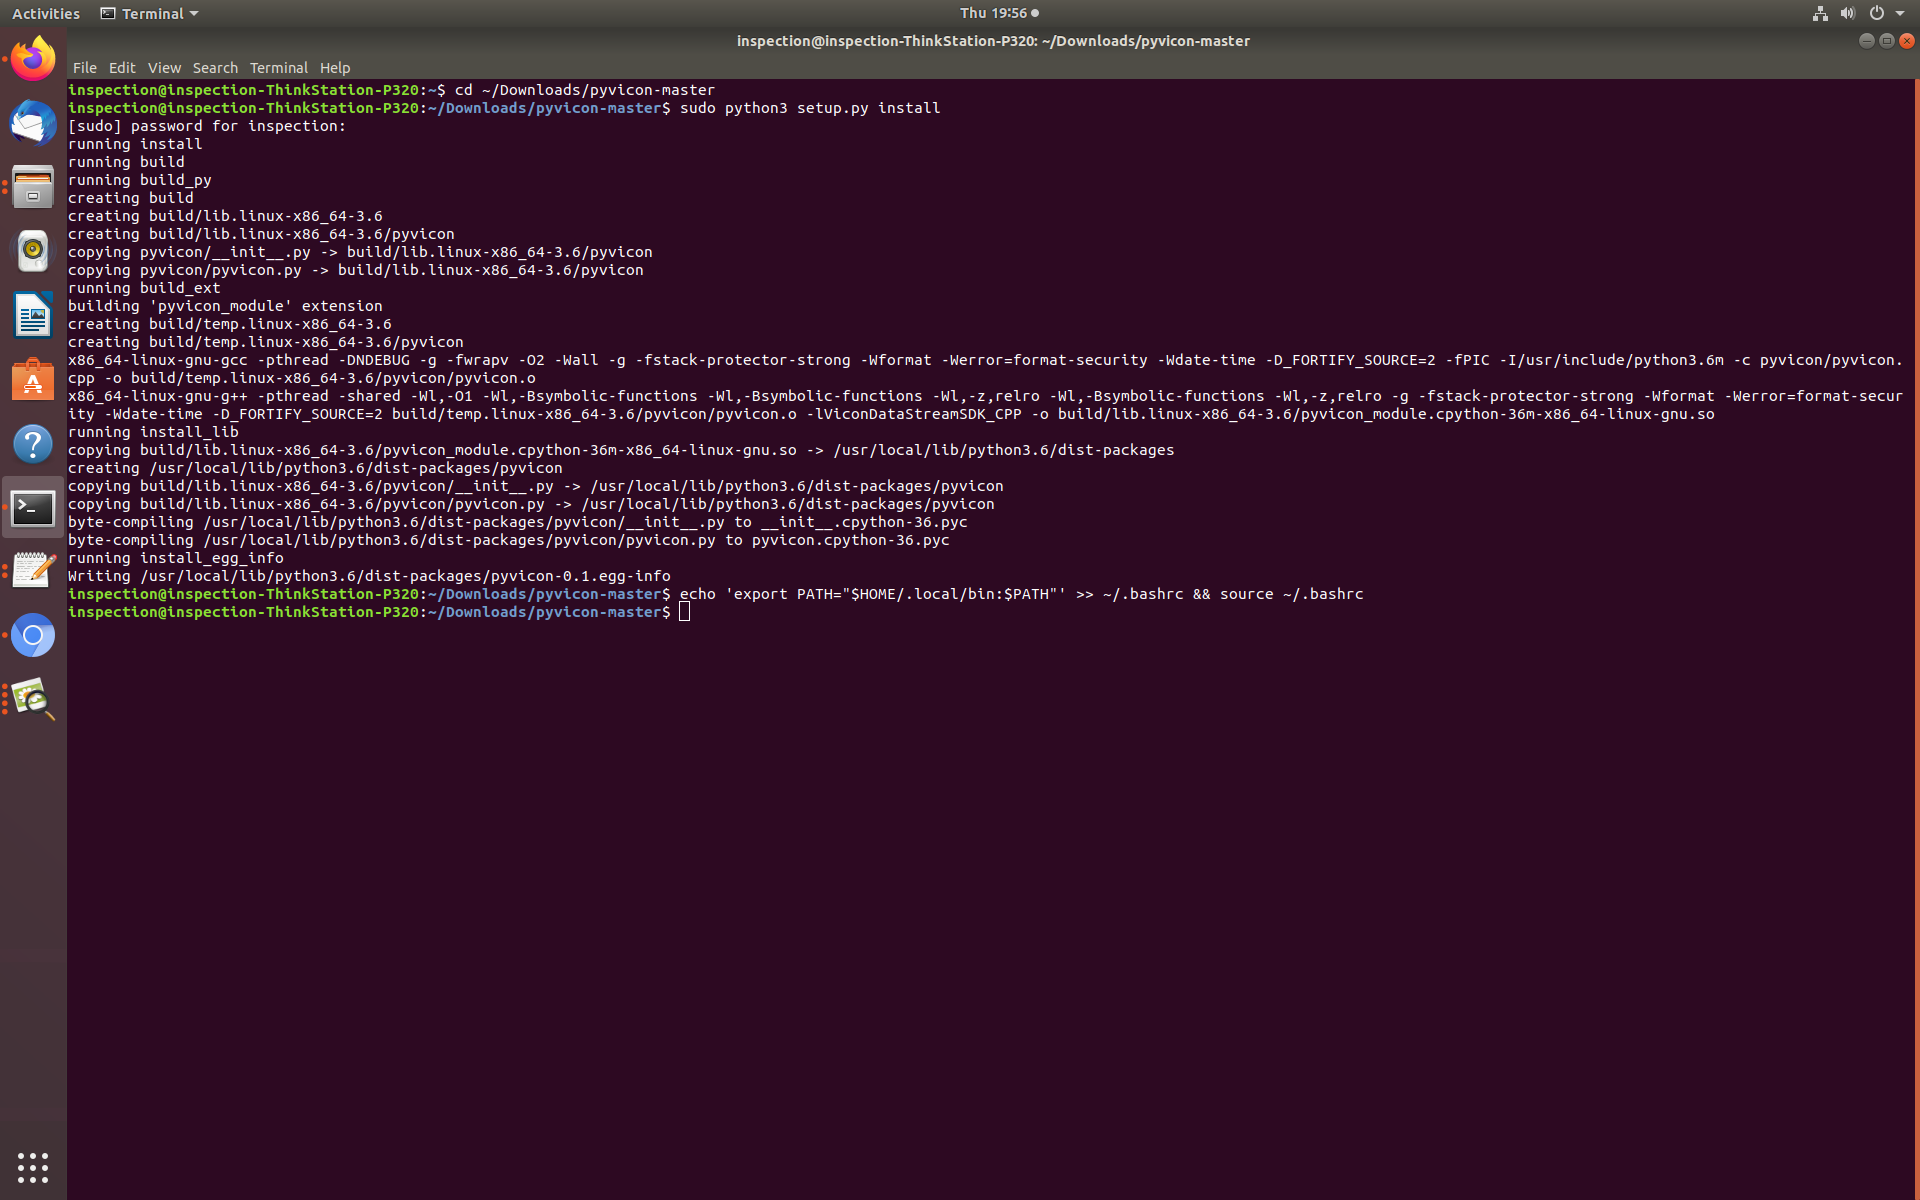
\includegraphics[width=1\linewidth]{pyvicon4.png}
    \caption{pyvicon setup and adding ~/local/bin to PATH}
    \label{fig:pyvicon4}
\end{figure}
\subsection{Installing Dependencies Packages}
A few dependencies are needed in order for pyvicon \& Mavproxy to work, run the following, which is seen in figure \ref{fig:setup9}: 
\begin{lstlisting}
    sudo apt-get install libgtk-3-dev 
    sudo apt remove modemmanager -y
    python3 -m pip install --user pathlib2
    python3 -m pip install --user matplotlib
    python3 -m pip install --user opencv-python
    python3 -m pip install --user Cython
    python3 -m pip install --user wxpython
\end{lstlisting}
Do note that this part is usually tricky as everyone's system has different versions of Python3, which inherently leads to different package that is supported with your version of Python3. For this step I recommend installing each package one by one, and troubleshooting whenever a package goes wrong. It is expected that you will have trouble with this step as I also had a lot of trouble when installing this in different computers. Refer to appendix A for common debugging solutions that has worked for me.
\begin{figure}[H]
    \centering
    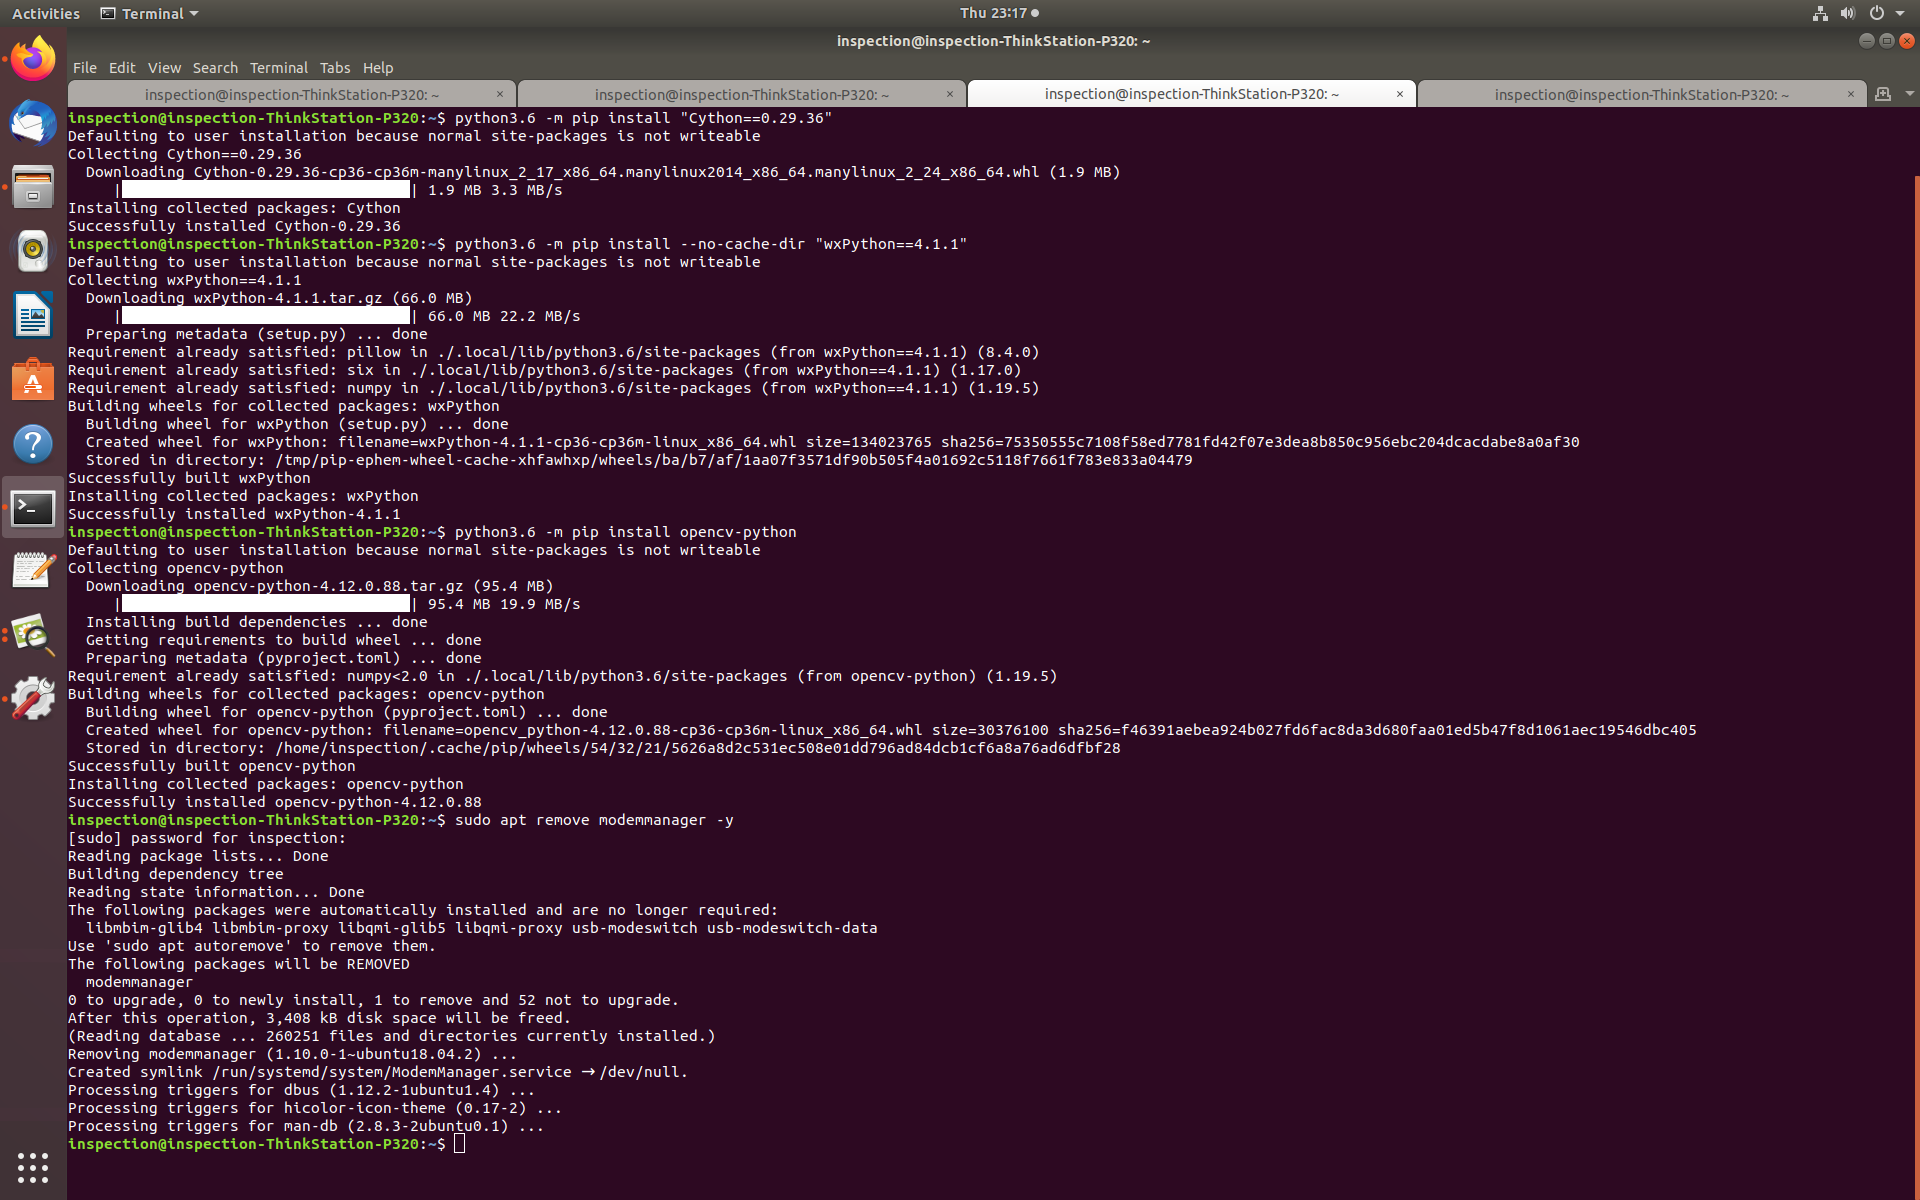
\includegraphics[width=1\linewidth]{setup9.png}
    \caption{Example of dependencies installation}
    \label{fig:setup9}
\end{figure}
\subsection{Hardware setup}
Once all dependencies are installed, musculoskeletally move towards the Host PC (Refer to 1st Guide \cite{matthew}) with your ground control station, locate the Vicon Ethernet Cable as shown in figure \ref{fig:hardware}. Connect the ethernet cable to your ground control station. 
\begin{figure}[H]
    \centering
    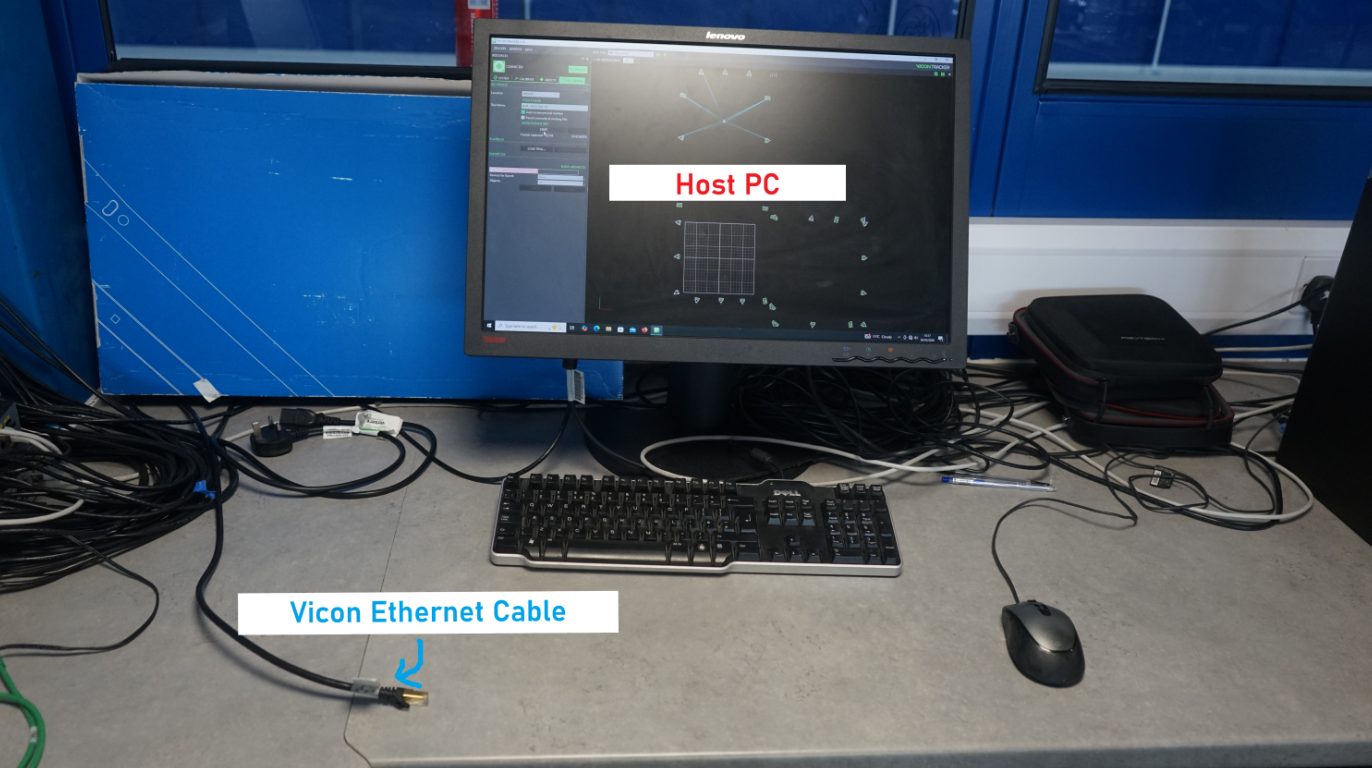
\includegraphics[width=1\linewidth]{Hardware photo.png}
    \caption{Photo of Vicon Ethernet Cable}
    \label{fig:hardware}
\end{figure}

\subsection{Network setup}
Once connected to the Ethernet cable, you will need to name your source of your Vicon positional data's ip address as \textit{vicon}, this can be done by typing this in Terminal, as shown in figure \ref{fig:network1}:\footnote{If you do some crawling around, you will note that this ethernet cable actually comes from within the flight arena, which would be useful if you want your GCS within the flight arena to test localisation later on.}
\begin{lstlisting}
    sudo nano /etc/hosts
\end{lstlisting}
\begin{figure}[H]
    \centering
    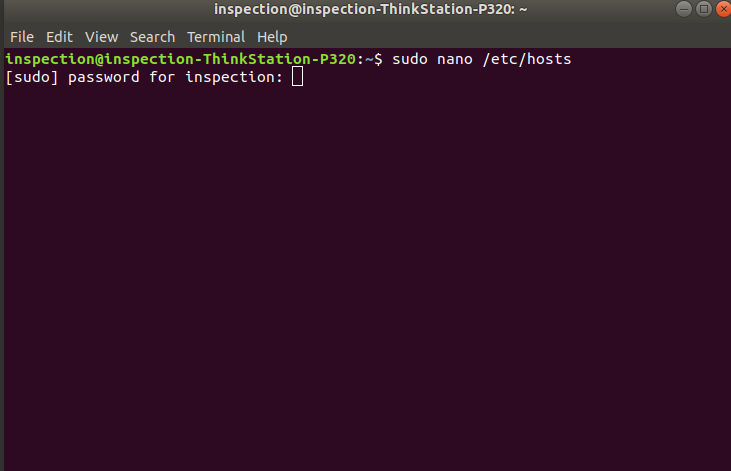
\includegraphics[width=0.8\linewidth]{network1.png}
    \caption{Code for network name editing}
    \label{fig:network1}
\end{figure}
A window will show up like figure \ref{fig:network2}
\begin{figure}[H]
    \centering
    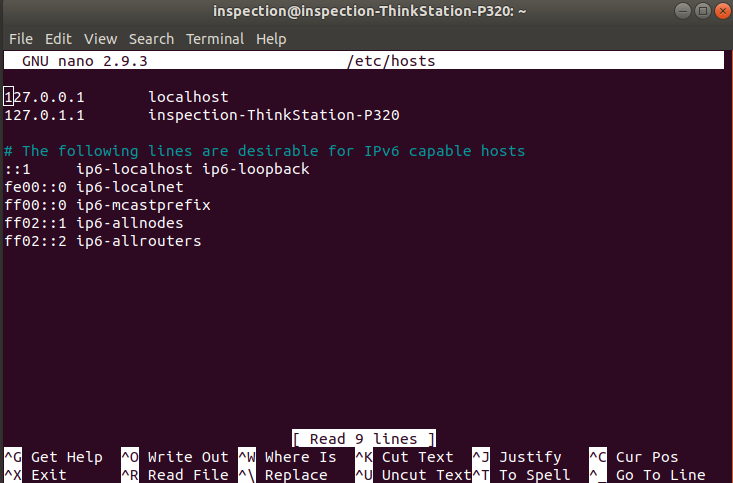
\includegraphics[width=0.8\linewidth]{network2.png}
    \caption{Enter Caption}
    \label{fig:network2}
\end{figure}
Add \textit{192.168.0.218 vicon} as shown in figure \ref{fig:network3}. Then press Ctrl+O to save the changes, Ctrl+X to exit the window. 
\begin{figure}[H]
    \centering
    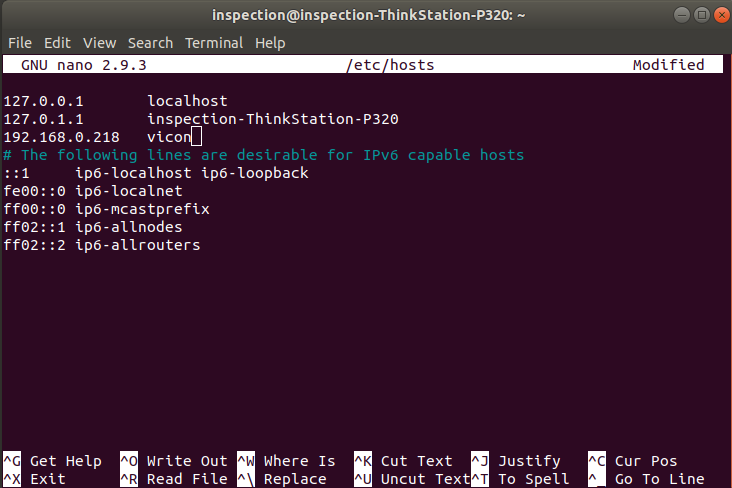
\includegraphics[width=0.8\linewidth]{network3.png}
    \caption{Enter Caption}
    \label{fig:network3}
\end{figure}
Test your connection to vicon vai ethernet cable by doing: 
\begin{lstlisting}
    ping vicon
\end{lstlisting}
If \textit{64 bytes from vicon (192.168.0.218): icmp\_seq=1 ttl=128 time=0.517ms} messages begin appearing like shown in figure \ref{fig:network5}, you have a correct connection between Vicon Tracker and your computer!
\begin{figure}[H]
    \centering
    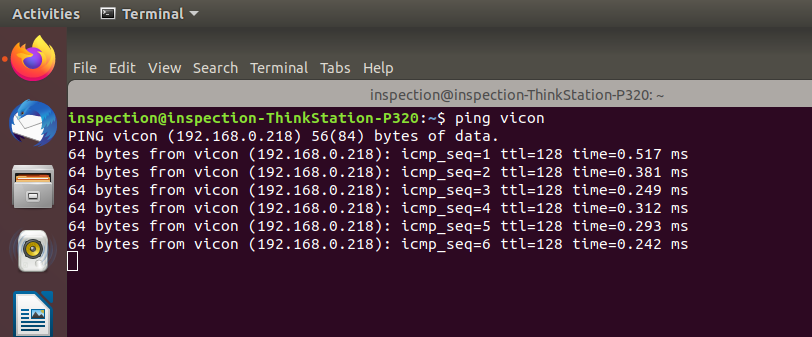
\includegraphics[width=0.8\linewidth]{network5.png}
    \caption{Enter Caption}
    \label{fig:network5}
\end{figure}
\subsection{Installing Mavproxy \& Mavlink}
Now (finally), we go into installation of Mavlink and Mavproxy. Run the following code as shown in figure \ref{fig:mavproxy11}: 
\begin{lstlisting}
    python3 -m pip install --upgrade --user pymavlink
    python3 -m pip install --upgrade --user mavproxy
\end{lstlisting}
\begin{figure}[H]
        \centering
        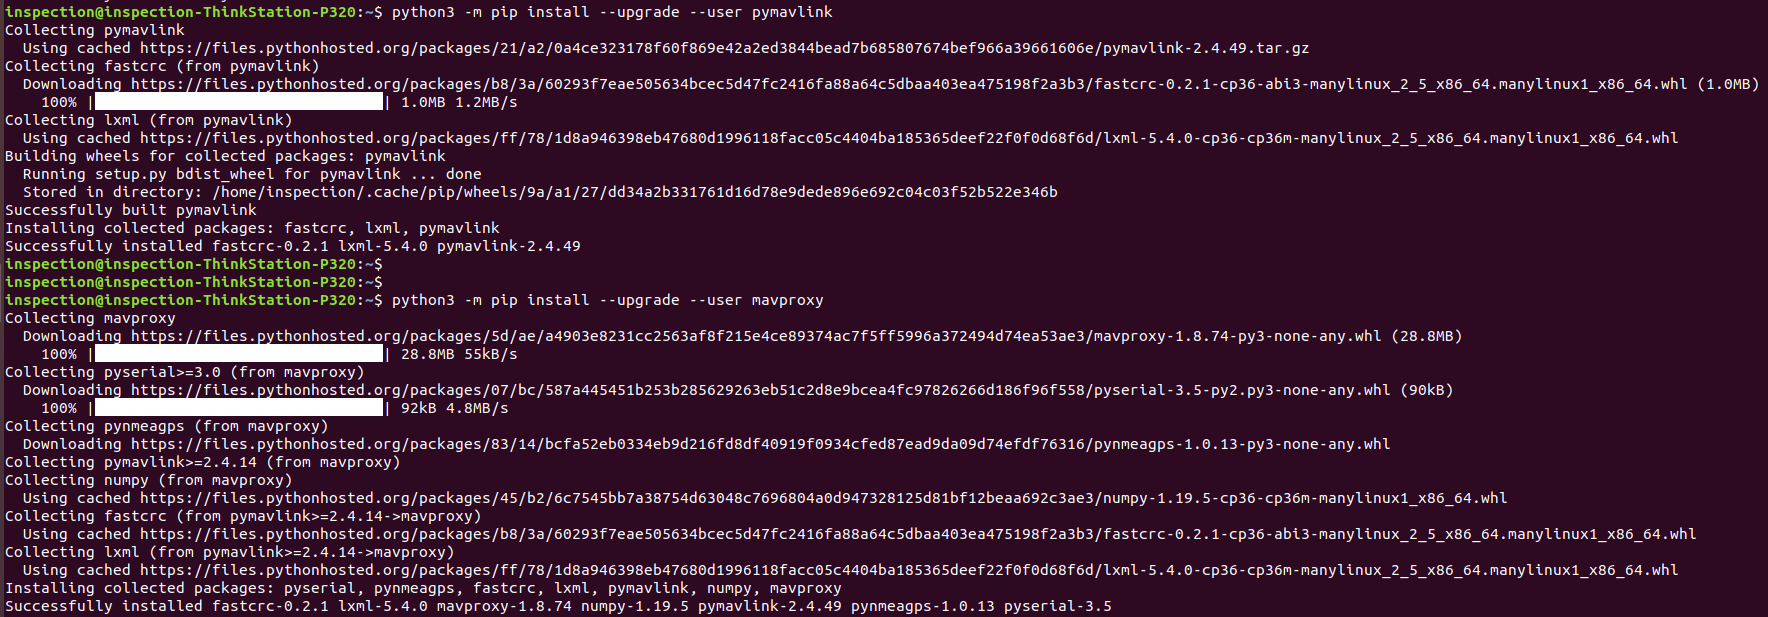
\includegraphics[width=1\linewidth]{mavproxy11.png}
        \caption{Installing Mavproxy and Mavlink}
        \label{fig:mavproxy11}
    \end{figure}
To test if your mavproxy installation is correct, run the following:

\begin{lstlisting}
    mavproxy.py --master :14550 --console --map
\end{lstlisting}

You should see the console and map window pops out as shown in figure \ref{fig:mavproxy2}. It will mention that link1 is down from the console but that is okay for now. Congrats! You should take a celebrative break now before continuing. Good job! 
\begin{figure}[H]
    \centering
    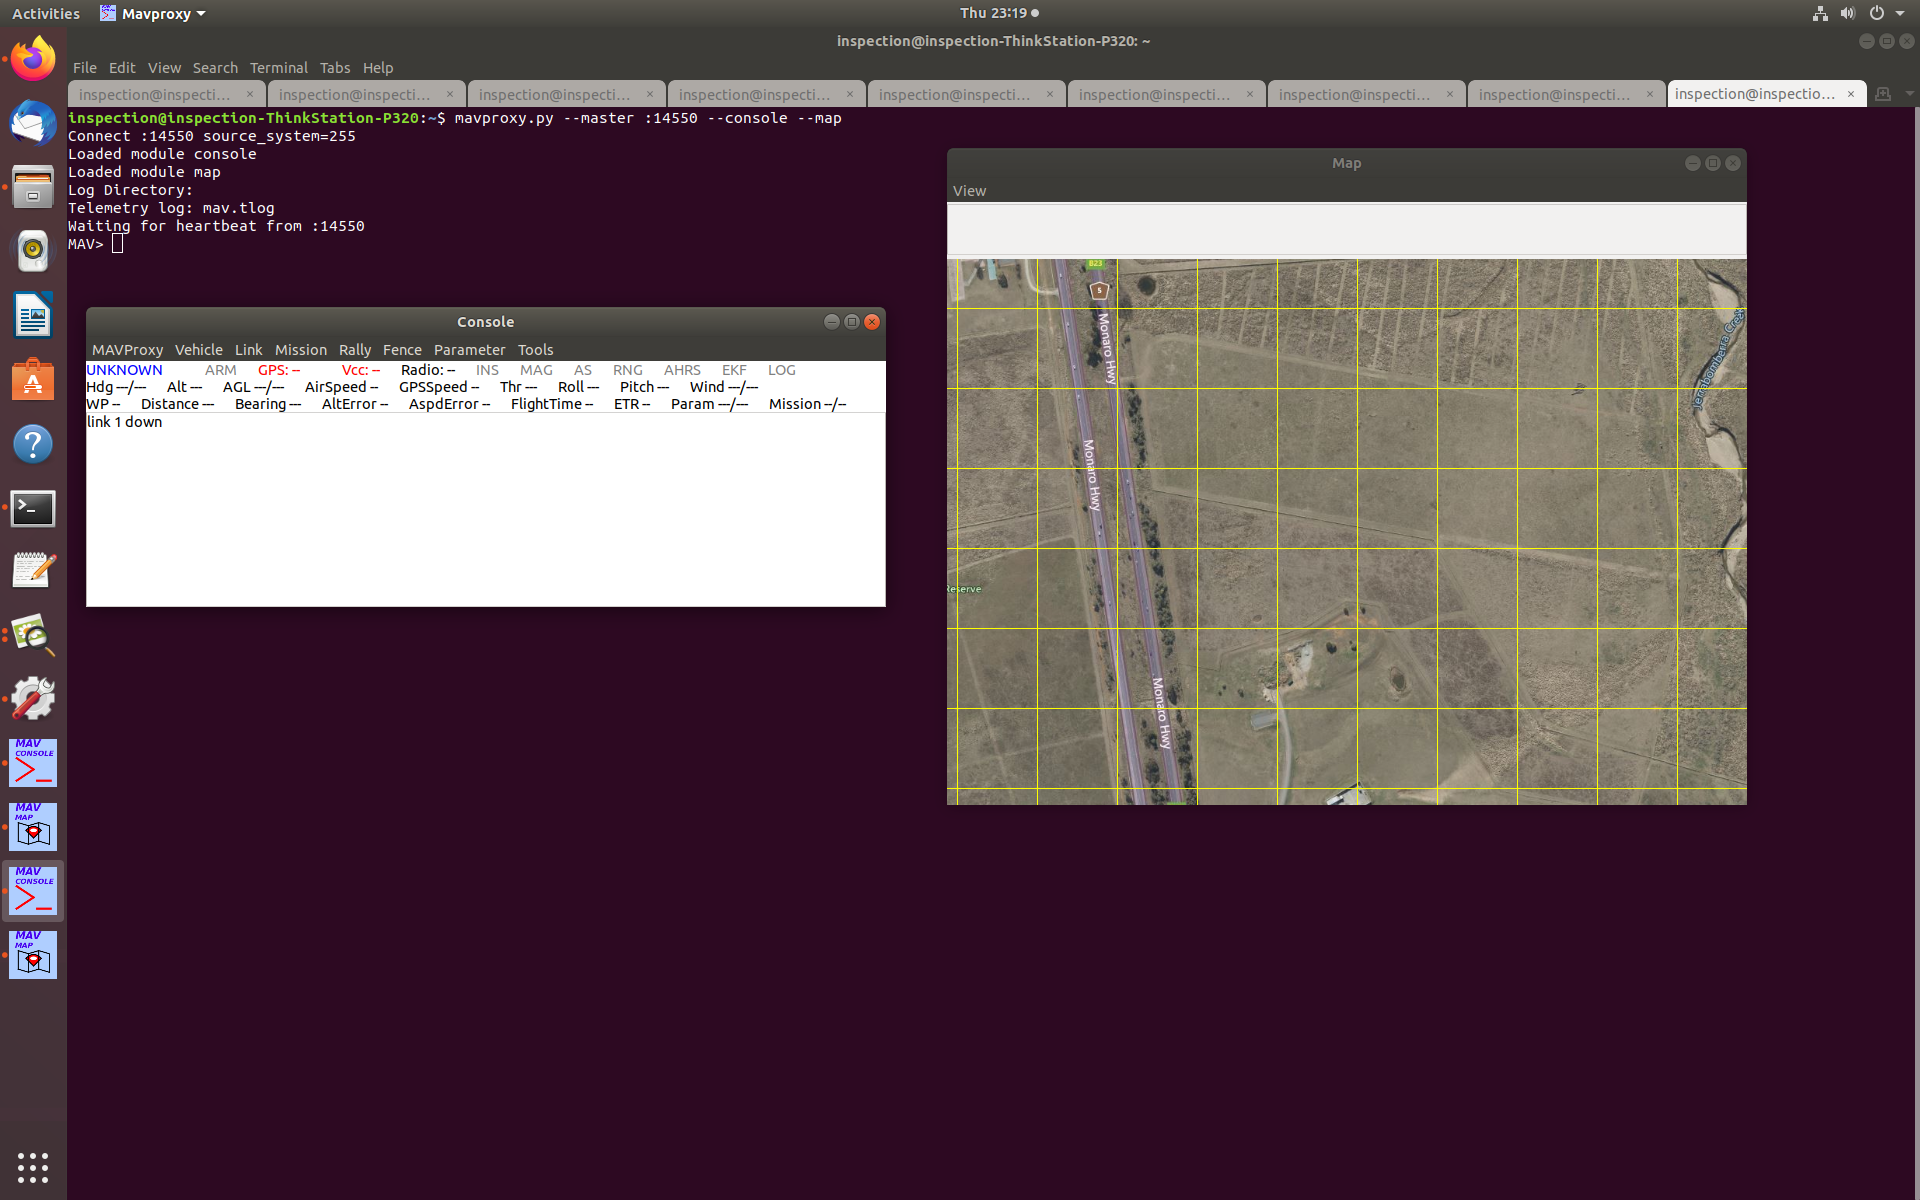
\includegraphics[width=1\linewidth]{mavproxy2.png}
    \caption{Enter Caption}
    \label{fig:mavproxy2}
\end{figure}

\subsection{Drone Setup}
You need to setup your drone so that you can host a wifi network for your ground control station to connect to. I used an ESP8266 wifi chip for this, althought you are more than welcome (encouraged even) to explore using host wifi features from raspberry pi, which is known to be more stable than the ESP8266. \cite{grace}

The flight controller I am using is the Pixhawk 6C, do note that not all Pixhawk works the same when setting up the serial port, so this is just an arbitary example given that works. 

Below is the pinout from \cite{engineeringprojects_esp8266}, courtesy to them for the image. 

\begin{figure}
    \centering
    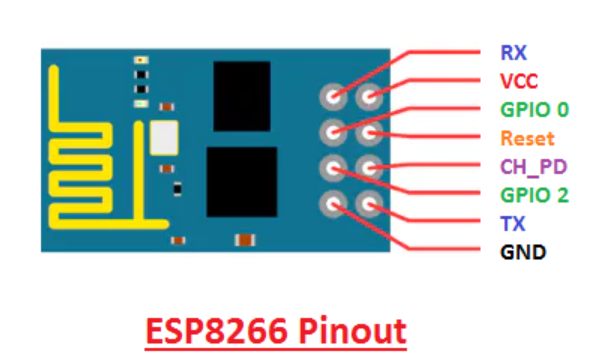
\includegraphics[width=0.6\linewidth]{pinout.png}
    \caption{Pinout for ESP8266}
    \label{fig:placeholder1}
\end{figure}

Connect the wiring to the Pixhawk.
\begin{figure}
    \centering
    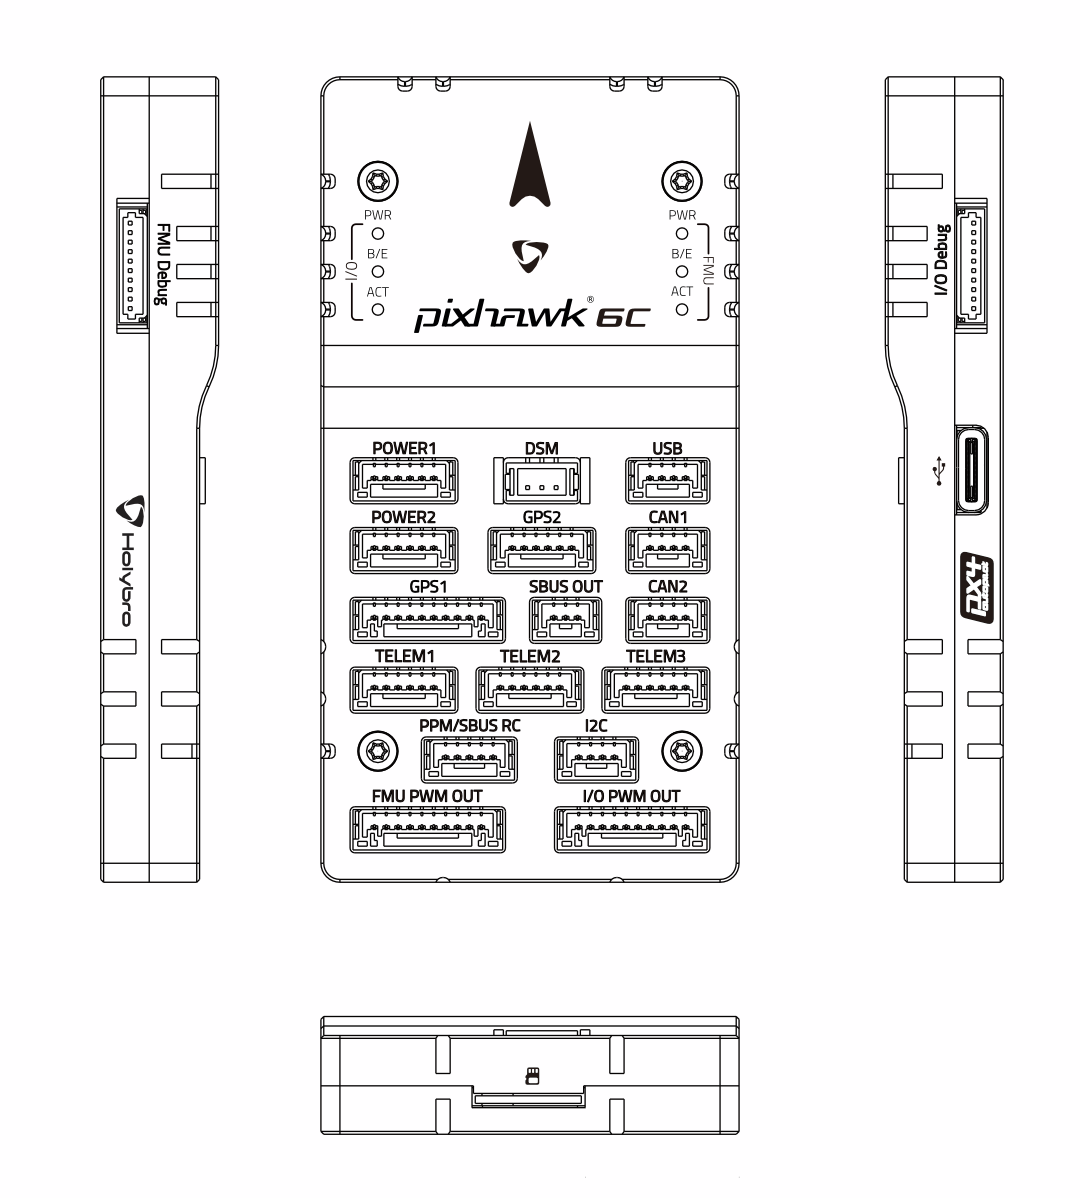
\includegraphics[width=1\linewidth]{pixhawk 6c.png}
    \caption{Enter Caption}
    \label{fig:placeholder2}
\end{figure}

\section{Communication Architecture}
\label{sec:comms}
The communication Architecture is primarily responsible for integrating different subsystems and ensure seamless data flows towards each subsystem. This section will mostly cover the development of 2 control stations to facilitate the communications, alongside other minor communication links established.\\

To begin with, the development of the Ground Control Station (GCS) focuses on integrating the Vicon Positioning System with the drone. The overall architecture starts with the Vicon Positioning system determining the drone’s position. It achieves that by using an assortment of cameras that track the infrared markers mounted on the drone at various locations and angles. The camera's data is then forwarded to a D-Link switch, which aggregates the camera feeds and sends them onwards to the Vicon Host PC; Inside the Host PC, the Vicon Tracker App processes the compiled IR footage to calculate the UAV’s pose, which results and output a pose data of the drone - broadcasting the positional data string via the Ethernet port. 

From that, the GCS connects to one of the Ethernet ports and recieves the positional data in real time. The GCS performs message reformatting from Vicon formatting into MAVLink protocol, which is described in detail below. Next, the GCS connects to a Wi‑Fi network hosted by the drone and transmits the positional data wirelessly in the form of GPS coordinates ($long \ , lat \ , z$). The drone uses this information to localise itself and carry out its mission. This cycle repeats continuously as the Vicon cameras track the drone’s IR markers and update its pose. An overall illustration of this communication flow is shown in Figure \ref{fig:comms_system}:
\begin{figure}[H]
    \centering
    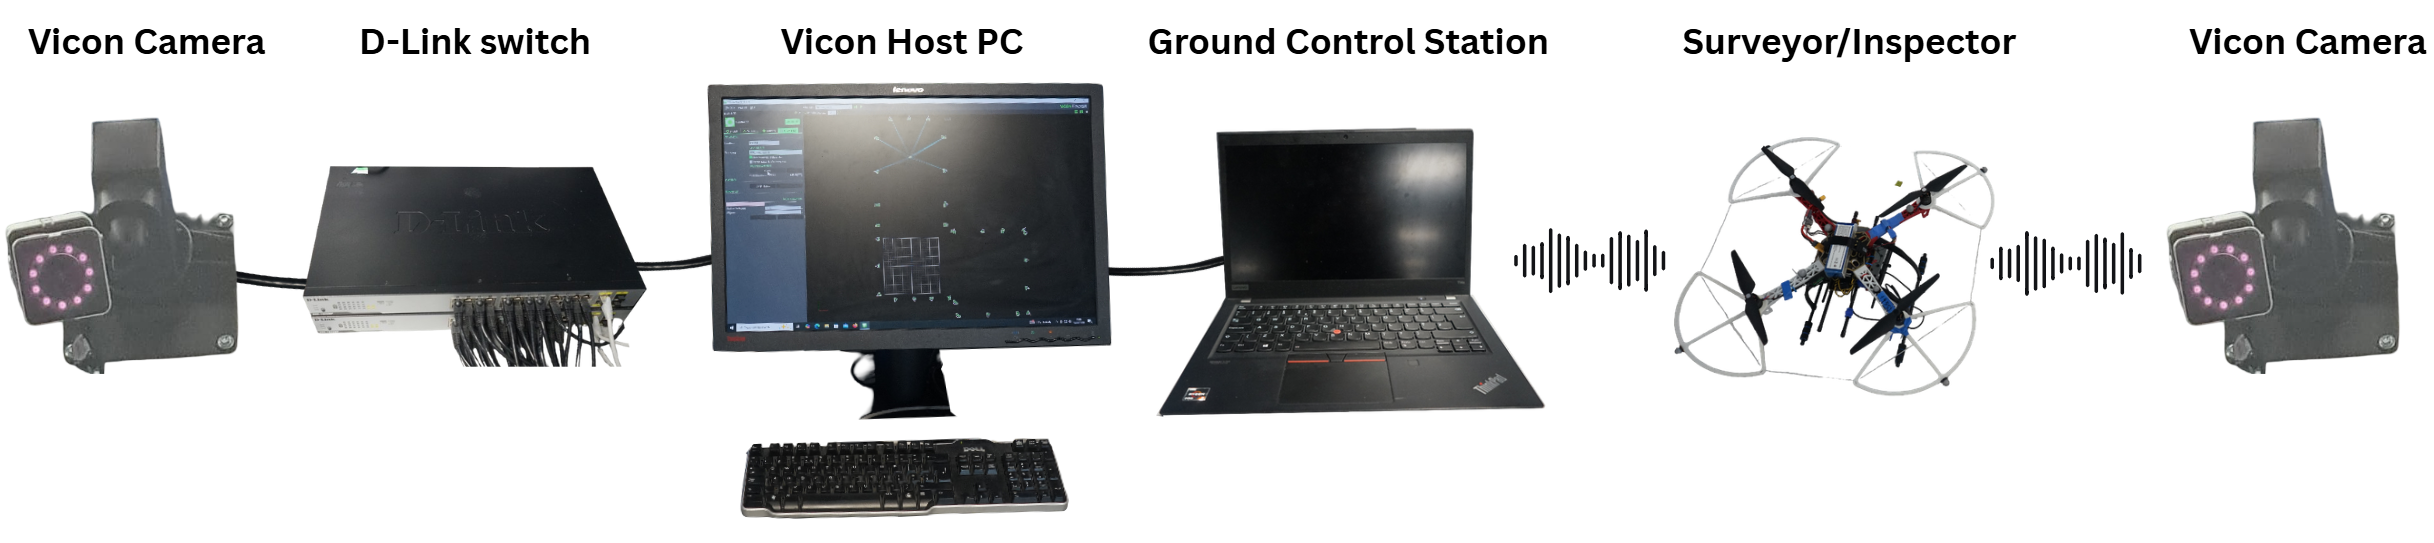
\includegraphics[width=1\linewidth]{Comms Arch.png}
    \caption{A high level flow diagram on the communication for localisation. }
    \label{fig:comms_system}
\end{figure}
The wireless telemetry is conducted with the use of an ESP8266 Wifi Module, jumped directly into the telemetry port of a Pixhawk6C flight controller, as seen in figure \ref{fig:ground2drone}
 
\begin{figure}[H]
    \centering
    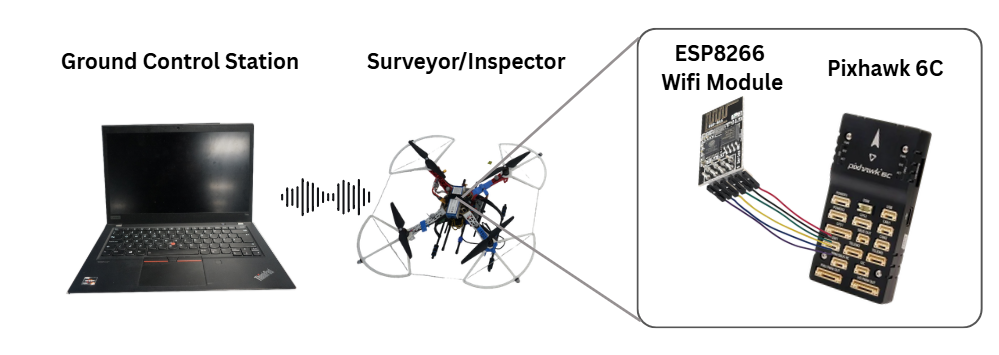
\includegraphics[width=0.8\linewidth]{Ground2Drone.png}
    \caption{Figure on The Wireless Communication Method between GCS and Drone.}
    \label{fig:ground2drone}
\end{figure}
The message conversion from Vicon to MAVLink is achieved using a combination of MavProxy (A command line driven Ground Control Station middleware developed by Ardupilot), the Vicon Software Development Kit (SDK), which enables parsing of the Vicon broadcast messages, and “PyVicon", an extension developed by MathGoron for MavProxy. Together, these software components convert the broadcasted Vicon data into injectable GPS coordinates that can be interpreted by the Pixhawk6C flight controller. A comprehensive guide and explanation are available in \cite{matthew}. A figure illustrating the software integration flow as described above is shown below in figure \ref{fig:GCS}:
\begin{figure}[H]
    \centering
    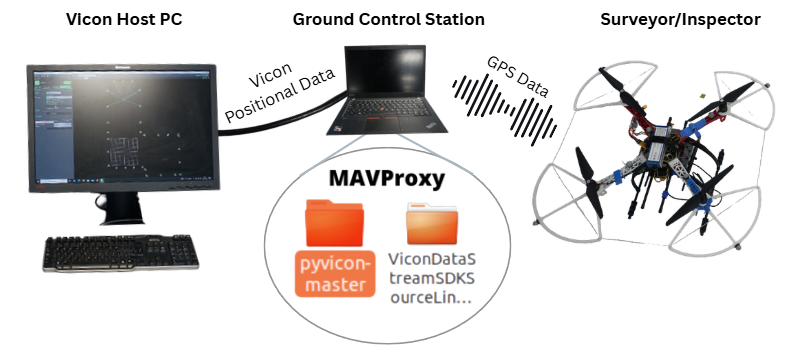
\includegraphics[width=0.8\linewidth]{GCS.png}
    \caption{Figure on the Software Integration in GCS.}
    \label{fig:GCS}
\end{figure}

The development of the Ground Mapping Station (GMS) is also included to integrate the mapping subsystem with the drone. Since onboard computers (a Raspberry Pi and a Jetson Nano) are used for sensor data acquisition (DAQ) and real time mapping is conducted in ROS Melodic, there is a need to activate these ROS nodes remotely. Secure Shell (SSH) is used to access the onboard computers’ terminals and, in turn, activate the corresponding DAQ and mapping nodes. A Local Area Network (LAN) router connects the Jetson Nano, Raspberry Pi, and Ground Mapping Station, as this network setup is required for SSH communication. Wi‑Fi connectivity is established for both the Inspector and Surveyor by using the Raspberry Pi 5’s built in wireless interface and an Intel 8265NGW Wi‑Fi module add on to the Jetson Nano. This setup is illustrated in figure \ref{fig:mapp} below:

\begin{figure}[H]
    \centering
    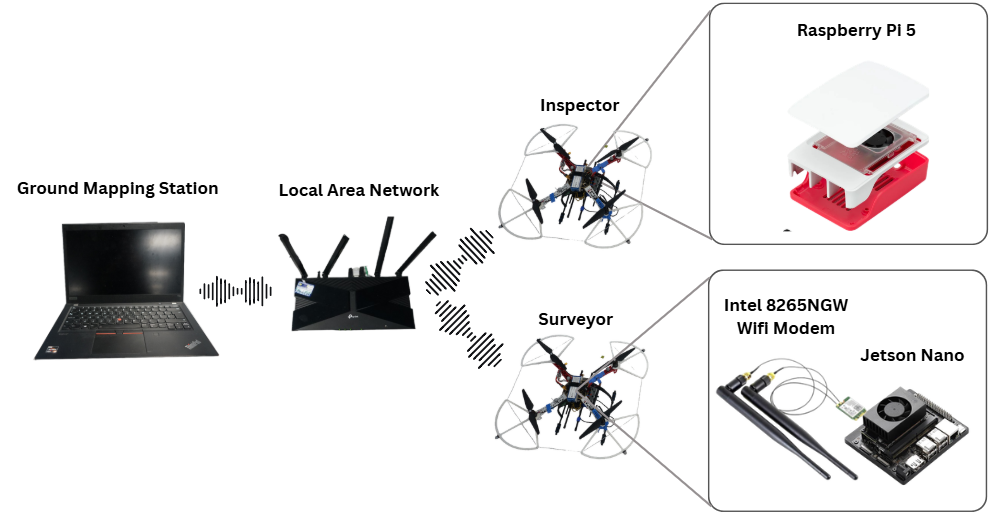
\includegraphics[width=1\linewidth]{Mapping detailed.png}
    \caption{An overall flow diagram on the communication for mapping.}
    \label{fig:mapp}
\end{figure}

The communication between the sensors, such as the depth camera and the Pi-Camera are established as follows. A simple USB serial interface is used to connect the depth camera to the Jetson Nano, whereas the Pi Camera utilized a flexible printed circuit to connect directly to the Raspberry Pi 5. ROS packages are then used for DAQ, which details is provided in later sections. A figure showing the sensors, their corresponding onboard computers, and their communication links is presented below in figure \ref{fig:sensors}.
\begin{figure}[H]
    \centering
    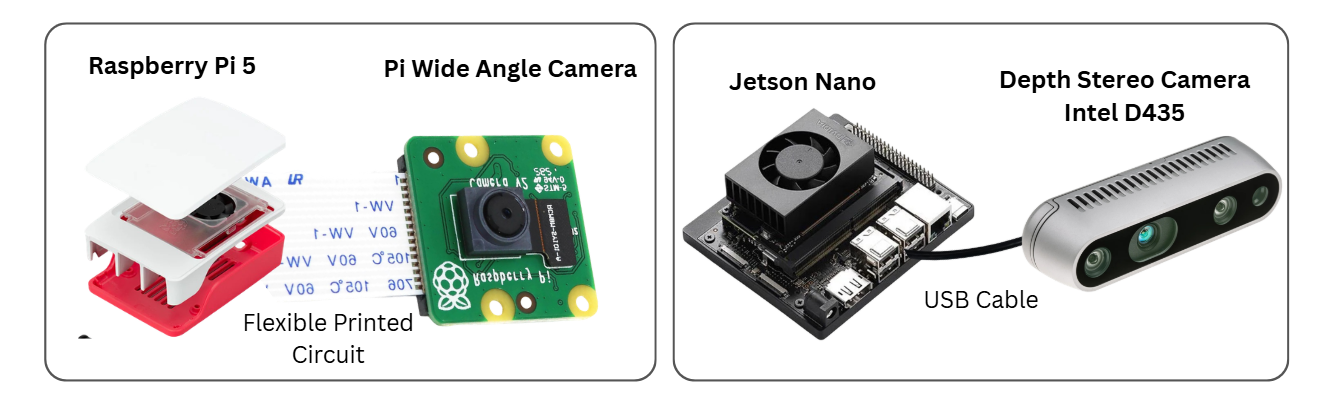
\includegraphics[width=1\linewidth]{Sensors.png}
    \caption{Onboard Computers and their corresponding communication link.}
    \label{fig:sensors}
\end{figure}
\subsection{Ardupilot setup}

\section{Operation Procedure}
\section{Concluding Remarks}
From this point, the Vicon Server should be tracking your now defined object! This information can be broadcasted through Ethernet cables and to your Ground Control Station via Robot Operating System (ROS) and corresponding ROS Package \textit{MAVPROXY} \& \textit{MAVLINK}, this is most likely your next step after this guide. This will be reflected in next edition of this report. (Which might be take a while, might be better if you start reading the Ardupilot guide yourself)\cite{ardupilot_vicon}. I hope this guide has been an useful resources towards your exciting projects!  
\section{Byspoke customisation and towards future tailoring - Nura Efendic}

\section{General Indoor Airmanship}
As I am mostly responsible for the teaching of how to use this lab, and inherently after this you will go flying. I have a responsibility to tell you how to properly fly inside the arena safely. 
\bibliographystyle{unsrt} % Orders references by citation order
\bibliography{bibliography}

\appendix
\section{}
If wxpython returns a source build error, it is possible that your python does not support the default installation version of wxpython, as I run python3.6 in this guide, the corresponding version that supports 3.6 is 4.1.1, I am able to download wxpython like the following: 
\begin{lstlisting}
    python3.6 -m pip install --no-cache-dir "wxpython==4.1.1"
\end{lstlisting}
Similarly for Cython, you can also specify versions of Cython if an error shows up: 
\begin{lstlisting}
    python3.6 -m pip install --no-cache-dir "Cython==0.29.36"
\end{lstlisting}
\textit{wxpython} takes a very long time to download, so it may look stale in terminal but it is actually installing, the installation stall usually looks like this in figure \ref{fig:pyvicon5}.
\footnote{If wxpython returns an source build error, this might be because of a mismatch in Python3 versions, this can be fixed by downloading a specific version of wxpython that matches your python3 version.}
\begin{figure}[H]
    \centering
    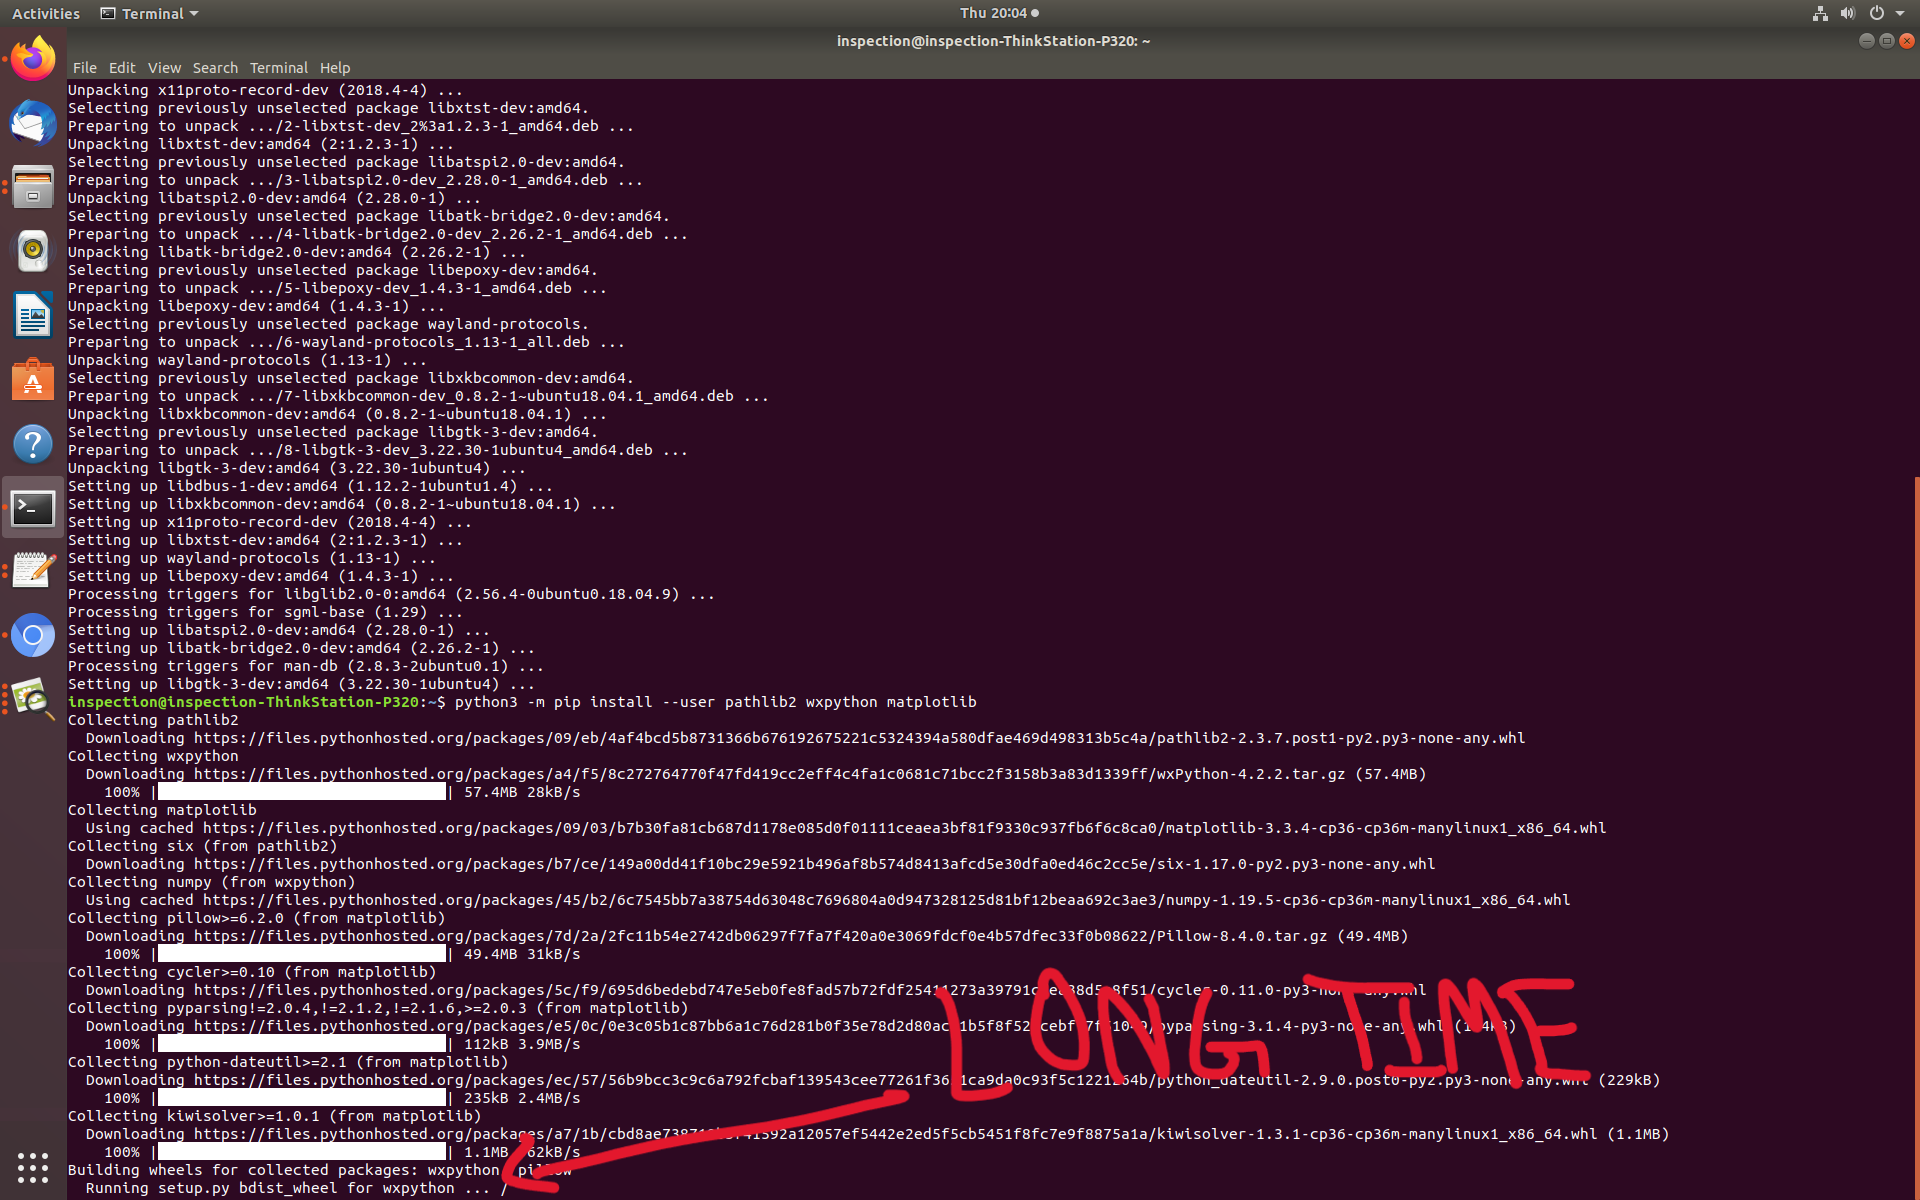
\includegraphics[width=1\linewidth]{pyvicon5.png}
    \caption{Visualization of wxpython and it's usual stall point}
    \label{fig:pyvicon5}
\end{figure}
testing
\end{document}
